%definira klasu dokumenta 
\documentclass[12pt]{report} 

%prostor izmedu naredbi \documentclass i \begin{document} se zove uvod. U njemu se nalaze naredbe koje se odnose na cijeli dokument

%osnovni LaTex ne može riješiti sve probleme, pa se koriste različiti paketi koji olakšavaju izradu željenog dokumenta
\usepackage[croatian]{babel} 
\usepackage{amssymb}
\usepackage{amsmath}
\usepackage{txfonts}
\usepackage{mathdots}
\usepackage{titlesec}
\usepackage{array}
\usepackage{lastpage}
\usepackage{etoolbox}
\usepackage{tabularray}
\usepackage{color, colortbl}
\usepackage{adjustbox}
\usepackage{geometry}
\usepackage[classicReIm]{kpfonts}
\usepackage{hyperref}
\usepackage{fancyhdr}

\usepackage{float}
\usepackage{setspace}
\usepackage{color}
\restylefloat{table}


\patchcmd{\chapter}{\thispagestyle{plain}}{\thispagestyle{fancy}}{}{} %redefiniranje stila stranice u paketu fancyhdr

%oblik naslova poglavlja
\titleformat{\chapter}{\normalfont\huge\bfseries}{\thechapter.}{20pt}{\Huge}
\titlespacing{\chapter}{0pt}{0pt}{40pt}


\linespread{1.3} %razmak između redaka

\geometry{a4paper, left=1in, top=1in,}  %oblik stranice

\hypersetup{ colorlinks, citecolor=black, filecolor=black, linkcolor=black,	urlcolor=black }   %izgled poveznice


%prored smanjen između redaka u nabrajanjima i popisima
\newenvironment{packed_enum}{
	\begin{enumerate}
		\setlength{\itemsep}{0pt}
		\setlength{\parskip}{0pt}
		\setlength{\parsep}{0pt}
	}{\end{enumerate}}

\newenvironment{packed_item}{
	\begin{itemize}
		\setlength{\itemsep}{0pt}
		\setlength{\parskip}{0pt}
		\setlength{\parsep}{0pt}
	}{\end{itemize}}




%boja za privatni i udaljeni kljuc u tablicama
\definecolor{LightBlue}{rgb}{0.9,0.9,1}
\definecolor{LightGreen}{rgb}{0.9,1,0.9}

%Promjena teksta za dugačke tablice
\DefTblrTemplate{contfoot-text}{normal}{Nastavljeno na idućoj stranici}
\SetTblrTemplate{contfoot-text}{normal}
\DefTblrTemplate{conthead-text}{normal}{(Nastavljeno)}
\SetTblrTemplate{conthead-text}{normal}
\DefTblrTemplate{middlehead,lasthead}{normal}{Nastavljeno od prethodne stranice}
\SetTblrTemplate{middlehead,lasthead}{normal}

%podesavanje zaglavlja i podnožja

\pagestyle{fancy}
\lhead{Programsko inženjerstvo}
\rhead{Iznajmi romobil}
\lfoot{Codeblaze}
\cfoot{stranica \thepage/\pageref{LastPage}}
\rfoot{\today}
\renewcommand{\headrulewidth}{0.2pt}
\renewcommand{\footrulewidth}{0.2pt}


\begin{document} 
	
	
	
	\begin{titlepage}
		\begin{center}
			\vspace*{\stretch{1.0}} %u kombinaciji s ostalim \vspace naredbama definira razmak između redaka teksta
			\LARGE Programsko inženjerstvo\\
			\large Ak. god. 2023./2024.\\
			
			\vspace*{\stretch{3.0}}
			
			\huge Iznajmi Romobil\\
			\Large Dokumentacija, Rev. \textit{1}\\
			
			\vspace*{\stretch{12.0}}
			\normalsize
			Grupa: \textit{Codeblaze}\\
			Voditelj: \textit{Marin Kvesić}\\
			
			
			\vspace*{\stretch{1.0}}
			Datum predaje: \textit{17.11.2023.}\\
	
			\vspace*{\stretch{4.0}}
			
			Nastavnik: \textit{Igor Stančin}\\
		
		\end{center}

	
	\end{titlepage}

	
	\tableofcontents


	\chapter{Dnevnik promjena dokumentacije}
		
		\textbf{\textit{Kontinuirano osvježavanje}}\\
				
		
		\begin{longtblr}[
				label=none
			]{
				width = \textwidth, 
				colspec={|X[2]|X[13]|X[3]|X[3]|}, 
				rowhead = 1
			}
			\hline
			\textbf{Rev.}	& \textbf{Opis promjene/dodatka} & \textbf{Autori} & \textbf{Datum}\\[3pt] \hline
			0.1 & Napravljen predložak.& Matija\newline Jakovac & 30.10.2023. 		\\[3pt] \hline 
			0.2	& Dodan opisa projekta.\newline Dodani obrasci uporabe i njihovi opisi. & Karla Šoštar, Katarina Đuroković, Matea Bušić  & 07.11.2023. 	\\[3pt] \hline 
			0.2.1 & Dodan ostatak obrazaca uporabe i njihovi opisi. & Karla Šoštar, Katarina Đuroković, Matea Bušić & 08.11.2023. \\[3pt] \hline 
			0.3 & Arhitektura i dizajn sustava & Mirna Knez & 08.11.2023. \\[3pt] \hline 
			0.4 & Ispravak obrazaca uporabe & Matea Bušić & 10.11.2023. \\[3pt] \hline 
			0.5 & Dodani zapisnici sastanaka & Matea Bušić & 11.11.2023. \\[3pt] \hline
			0.6 & Popravak baze podataka & Mirna Knez & 12.11.2023. \\[3pt] \hline
			0.9 & Dodani funkcionalni zahtjevi & Matea Bušić & 13.11.2023. \\[3pt] \hline 
			0.10 & Dodani dijagrami razreda & Mirna Knez & 14.11.2023. \\[3pt] \hline 
			0.10.1 & Ispravak obrazaca uporabe & Karla Šoštar, Katarina Đuroković, Matea Bušić & 15.11.2023. \\[3pt] \hline 
			0.11 & Dodani sekvencijski dijagrami i dijagrami obrazaca uporabe & Karla Šoštar, Katarina Đuroković & 17.11.2023. \\[3pt] \hline 
			1.0 & Završna verzija za prvu reviziju & Matea Bušić & 17.11.2023. \\[3pt] \hline
			1.1 & Dodan dijagram razmještaja & Mirna Knez & 11.01.2024. \\[3pt] \hline
			1.2 & Dodane upute za puštanje u pogon & Mirna Knez & 15.01.2024. \\[3pt] \hline
			1.3 & Dodan zaključak i budući rad & Matea Bušić & 15.01.2024. \\[3pt] \hline
			1.4 & Dodani sastanci u Dnevnik sastajanja  & Matea Bušić & 16.01.2024. \\[3pt] \hline
			1.5 & Dodan dijagram stanja i dijagram aktivnosti & Katarina Đuroković & 16.01.2024. \\[3pt] \hline
			1.6 & Popravak dijagrama razreda & Katarina Đuroković & 16.01.2024. \\[3pt] \hline
			1.7 & Dodani testovi & Karla Šoštar & 17.01.2024. \\[3pt] \hline 
			1.8 & Dodan dijagram komponenti & Matea Bušić & 19.01.2024. \\[3pt] \hline 
		\end{longtblr}
	
	
	
	\chapter{Opis projektnog zadatka}
		
		Cilj ovog projekta je razviti programsku podršku za stvaranje web aplikacije „Iznajmi romobil“ koja će korisnicima omogućiti da iznajme svoj električni romobil u periodima dana kada ga ne koriste. Aplikacija će korisnicima omogućavati brz i jednostavan pristup električnim romobilima dostupnima za najam kao i postavljanje ponude za iznajmljivanje svog romobila. Korisnici će moći za vrijeme kada su na poslu, kavi, treningu i slično odnosno kada ne koriste svoj električni romobil isti iznajmiti. Prilikom postavljanja ponude oni će odrediti gdje i do kada romobil mora biti vraćen. U slučaju da romobil ne bude vraćen na vrijeme, klijentu se naplaćuje naknada određena od strane iznajmljivača. Klijent će na temelju ponuđenih romobila i informacija o njima odabrati onaj koji je u tom trenutku dostupan i najviše odgovara njegovim potrebama. Funkcionalnosti aplikacije ovisiti će o vrsti korisnika. Aplikacija ima četiri vrste korisnika: neregistriranog korisnika, klijenta, iznajmljivača i administratora. S tim da isti korisnik može istovremeno biti i iznajmljivač i klijent.
		\newline 
		\newline
		Prilikom pokretanja aplikacije korisnicima se neovisno o tome jesu li prijavljeni ili ne prikazuje popis svih aktivnih ponuda romobila. Neregistrirani korisnici mogu pregledavati trenutno dostupne romobile i njihova cijene, ali ih ne mogu iznajmiti. Nakon što se prijave ili kreiraju novi korisnički račun, ponuđeni romobili im postaju dostupni za najam. Prilikom kreiranja novog računa korisnici moraju unijeti sljedeće podatke:
		
		\begin{packed_item}
			\item \textit{ime i prezime}
			\item \textit{email adresa}
			\item \textit{nadimak}
			\item \textit{broj kartice}
		\end{packed_item}
		
		Osim navedenog, korisnici prilikom registracije moraju dostaviti kopiju osobne iskaznice i potvrdu o nekažnjavanju. Nakon što su svi potrebni dokumenti dostavljeni, administrator pregledava dokumente te odobrava ili odbija registraciju. Dok administrator ne odobri registraciju, korisnik se ne može prijaviti u sustav. Kada mu administrator odobri registraciju, korisnik se prijavljuje u sustav. Ako korisnik prilikom unosa podataka za prijavu unese podatke koji ne odgovaraju nijednom registriranom korisniku u bazi, šalje mu se obavijest o neispravnosti podataka. BLOK U slučaju da administrator odbije zahtjev za registraciju zbog neispravnosti dostavljenih dokumenata, korisnik može ponovno predati dokumente. Svaki klijent u aplikaciji može pogledati svoj profil na kojem se nalaze njegovi osobni podaci te urediti isti odabirom opcije "Uredi profil".  Ako pri uređivanju profila dođe do unošenja podataka u neispravnom obliku, korisnik dobiva obavijest o neispravnosti. Nakon unosa promjena, korisnik mora odabrati opciju "Spremi promjene" kako bi potvrdio pohranjivanje promjena u bazu podataka. Administrator ima pravo blokirati korisnika odnosno zabraniti mu pristup aplikaciji odabirom opcije "Blokiraj korisnika". Za takvog se korisnika u bazu podataka upisuje da je blokiran te će mu pri sljedećoj prijavi biti onemogućen pristup sustavu. Iznajmljivač je korisnik koji postavlja svoj romobil u aplikaciju za iznajmljivanje. On prilikom registracije romobila unosi podatke o romobilu i postavlja sliku romobila koja dokazuje njegovo trenutno stanje. Prilikom postavljanja ponude za iznajmljivanje, iznajmljivač unosi trenutnu lokaciju romobila, lokaciju na koju želi da se romobil vrati, vrijeme do kada romobil mora biti vraćen, cijenu iznajmljivanja po prijeđenom kilometru te iznos novčane kazne u slučaju da romobil ne bude vraćen na vrijeme. Ako je neki romobil dostupan za iznajmljivanje, iznajmljivač oglas može objaviti i na nekoj društvenoj mreži odabirom opcije "Objavi na društvenu mrežu". Svaki iznajmljivač na svom profilu može pregledavati svoje registrirane romobile te ih brisati. Unutar aplikacije dostupna je mogućnost izmjenjivanja poruka korisnika. Klijent se, kada odabere romobil koji želi iznajmiti, javlja iznajmljivaču s porukom i zahtjevom za iznajmljivanje. Iznajmljivač pregledava zahtjeve za iznajmljivanje te tada može prihvaća ili odbija ponudu. Nakon što prihvati ponudu, klijentu se šalje obavijest da je iznajmljivanje odobreno i oglas se briše. Klijent prije pokretanja romobila provjerava odgovara li fotografija romobila njegovom stvarnom stanju. Ako ne odgovara, on ima mogućnost odabirom opcije "Zamijeni sliku" zamijeniti sliku romobila novom slikom i kratkim opisom o razlikama između nove i stare slike. Kada klijent zamijeni sliku, iznajmljivaču se šalje obavijest o zamjeni slika. On tada administratoru može poslati žalbu na zamjenu slika ukoliko smatra da klijentova slika ne odgovara stvarnom stanju romobila. Administrator nakon zaprimanja žalbe pregledava slike i odabire onu koja će se pohraniti u bazu. Nakon što administrator donese odluku, klijentu i iznajmljivaču se šalje obavijest o donesenoj odluci. Na kraju iznajmljivanja, klijent vraća romobil i u aplikaciji potvrđuje da ga je vratio. Nakon toga slijedi provjera je li romobil vraćen u pravo vrijeme te se izračunava cijena koju klijent mora platiti. Klijent i iznajmljivač dobivaju obavijest da je iznajmljivanje završeno i cijenu iznajmljivanja koju klijent treba platiti iznajmljivaču. Transakcija se izvršava i sprema u bazu podataka. Po završetku iznajmljivanja, iznajmljivač može ocijeniti klijenta i napisati komentar. Sve ocjene i komentari za pojedinog klijenta vidljivi su na njihovim profilima koje ostali korisnici mogu pregledavati. 
		
		
		
		
		
		
	
	\chapter{Specifikacija programske potpore}
		
	\section{Funkcionalni zahtjevi}
			
			
			
			\noindent \textbf{Dionici:}
			
			\begin{packed_enum}
				
				\item Klijenti
				\item Iznajmljivači			
				\item Administratori sustava
				\item Razvojni tim 
				
			\end{packed_enum}
			
			\noindent \textbf{Aktori i njihovi funkcionalni zahtjevi:}
			
			
			\begin{packed_enum}
				\item  \underbar {Neregistrirani korisnik/posjetilac (inicijator) može:}
				
				\begin{packed_enum}
					
					\item pregledavati dostupne romobile
					\item odabrati romobil da dobije detaljnije podatke o njemu
					\item registrirati se u sustav, stvoriti novi korisnički račun
					
					
				\end{packed_enum}
			
				\item  \underbar{Klijent (inicijator) može:}
				
				\begin{packed_enum}
					\item pregledavati dostupne romobile
					\item pregledati osobne podatke na svome profilu i urediti ih 
					\item izbrisati svoj profil
					\item registrirati romobil
					\item iznajmiti romobil
					\item zamijeniti sliku romobila
					\item vratiti romobil
					\item pregledati svoje prethodne transakcije
					\item pogledati profil drugog korisnika
					\item pogledati razgovor s nekim drugim korisnikom
					\item poslati poruku drugom korisniku
					\item izbrisati razgovor s drugim korisnikom
					
				
					
				\end{packed_enum}
				\item  \underbar {Iznajmljivač (inicijator) može:}
				
				\begin{packed_enum}
				\item pogledati detaljne informacije o svom registriranom romobilu
				\item promijeniti informacije o registriranom romobilu
				\item izbrisati registrirani romobil
				\item postaviti oglas za registrirani romobil
				\item objaviti oglas za iznajmljivanje romobila na društvene mreže
				\item pregledati i uređivati svoj oglas
				\item izbrisati oglas za iznajmljivanje romobila
				\item prihvatiti ili odbiti zahtjev za iznajmljivanje
				\item poslati žalbu na zamjenu slika romobila 
				\item ocijeniti klijenta
				\item izbrisati svoju recenziju o drugom korisniku
				
			\end{packed_enum}
			\item  \underbar {Administrator (inicijator) može:}
			
			\begin{packed_enum}
		
			\item pregledati dostupne romobile i detalje o njima
			\item pregledati dokumentaciju za registraciju i prihvatiti ili odbiti zahtjev za registraciju
			\item pregledati svoj profil
			\item urediti svoj profil
			\item izbrisati svoj profil
			\item Izbrisati oglas
			\item odlučiti poništava li se zamjena slika ili ne
			\item pogledati profil drugog korisnika
			\item izbrisati recenziju o nekom korisniku
			\item blokirati korisnika
			\item odblokirati korisnika
			\item dodati drugom korisniku ulogu administratora
			\item oduzeti drugom administratoru ulogu administratora
			
			
		
			
			\end{packed_enum}
			\item  \underbar {Baza podataka(sudionik):}

			\begin{packed_enum}
				
				\item pohranjuje sve podatke o korisnicima i njihovim ovlastima
				
				\item pohranjuje sve podatke o romobilima, njihovim iznajmljivanjima i transakcijama
				
				
				
			\end{packed_enum}
			
			\item  \underbar {Banka (inicijator) može:}
			
			\begin{packed_enum}
				
			\item umanjiti iznos novca na računu klijenta za iznos cijene iznajmljivanja
			
			\item uplati cijenu iznajmljivanja iznajmljivaču na račun
			
			
			
			\end{packed_enum}
		\end{packed_enum}
			
			\eject 
			
			
				
			\subsection{Obrasci uporabe}
				
			
				
				\subsubsection{Opis obrazaca uporabe}
					
					
					\noindent \underbar{\textbf{UC1 - Pregledaj romobil}}
					\begin{packed_item}
	
						\item \textbf{Glavni sudionik: }Neregistrirani korisnik, klijent, administrator 
						\item  \textbf{Cilj:} Pregledati dostupne romobile i detalje o njima i ponudi
						\item  \textbf{Sudionici:} Baza podataka
						\item  \textbf{Preduvjet:} -
						\item  \textbf{Opis osnovnog tijeka:}
						
						\item[] \begin{packed_enum}
	
							\item Prilikom učitavanja aplikacije prikazuju se romobili dostupni za iznajmljivanje
							\item Korisnik pronalazi i odabire željeni romobil
							\item Korisniku se prikazuju detaljnije informacije o romobilu i uvjetima iznajmljivanja
						
						\end{packed_enum}
					\end{packed_item}
						
						\noindent \underbar{\textbf{UC2 - Registriraj se}}
						\begin{packed_item}
							
							\item \textbf{Glavni sudionik: } Neregistrirani korisnik
							\item  \textbf{Cilj:} Napraviti korisnički račun kojim se pristupa sustavu
							\item  \textbf{Sudionici:} Administrator, baza podataka
							\item  \textbf{Preduvjet:} -
							\item  \textbf{Opis osnovnog tijeka:}
							
							\item[] \begin{packed_enum}
								
								\item	Neregistrirani korisnik odabire opciju „Registriraj se“
								\item 	Neregistriranom korisniku prikazuje se stranica za registraciju
							    \item 	Neregistrirani korisnik unosi podatke za registraciju
								\item 	Unesena kopija osobne iskaznice i potvrda o nekažnjavanju šalju se administratoru na pregled
								\item 	Stvara se novi korisnički račun čiji se podatci pohranjuju u bazu podataka
								\item 	Neregistriranom korisniku se prikazuje stranica za prijavu
								
								 
								
							\end{packed_enum}
							
							\item  \textbf{Opis mogućih odstupanja:}
							
							\item[] \begin{packed_item}
								
								\item[3.a] Unos podataka u nedozvoljenom formatu ili unos već zauzetog nadimka ili e-mail adrese
								\item[] \begin{packed_enum}
									
									\item 	Neregistrirani korisnik dobiva odgovarajuću obavijest o neispravnosti podataka
									\item	Neregistrirani korisnik mijenja potrebne podatke i završava s unosom ili odustaje od registracije
									
									
								\end{packed_enum}
								
								
							\end{packed_item}
						\end{packed_item}
						\noindent \underbar{\textbf{UC3 - Odobri ili odbij registraciju}}
						\begin{packed_item}
							
							\item \textbf{Glavni sudionik: } Administrator
							\item  \textbf{Cilj: } Odlučiti o valjanosti kopije osobne iskaznice i potvrde o nekažnjavanju
							\item  \textbf{Sudionici: }Klijent, baza podataka
							\item  \textbf{Preduvjet: }Postoji barem jedan zahtjev za registraciju 
							\item  \textbf{Opis osnovnog tijeka:}
							
							\item[] \begin{packed_enum}
								
								\item Administrator pregledava dokumentaciju poslanu pri registraciji korisnika ili pri ponovnom slanju dokumentacije 
								\item Administrator odlučuje o potvrđivanju dokumenata i njegova odluka se zapisuje u bazu podataka
								\item Klijenta čija se registracija provjerava se preusmjerava na stranicu za prijavu
								
								
							\end{packed_enum}
						\end{packed_item}
						\noindent \underbar{\textbf{UC4 - Ponovno predaj dokumente}}
						\begin{packed_item}
							
							\item \textbf{Glavni sudionik: }Neregistrirani korisnik
							\item  \textbf{Cilj:} Ponovno predati kopiju osobne iskaznice i potvrdu o nekažnjavanju na pregled
							\item  \textbf{Sudionici:} Administrator, baza podataka
							\item  \textbf{Preduvjet:} Prethodno odbijen zahtjev za registraciju
							\item  \textbf{Opis osnovnog tijeka:}
							
							\item[] \begin{packed_enum}
								
								\item Neregistrirani korisnik unosi novu dokumentaciju za registraciju u sustav 
								\item Dokumentacija se šalje administratoru na pregled 
								\item Neregistriranom korisniku se prikazuje stranica za čekanje odobrenja registracije
								
								
							\end{packed_enum}
							
							\item  \textbf{Opis mogućih odstupanja:}
							
							\item[] \begin{packed_item}
								
								\item[1.a] Unos dokumentacije u nedozvoljenom formatu 
								\item[] \begin{packed_enum}
									
									\item Neregistrirani korisnik dobiva odgovarajuću obavijest o neispravnosti podataka  
									\item Neregistrirani korisnik ispravno unosi dokumentaciju i završava s unosom ili odustaje od ponovne predaje dokumentacije  
									
								\end{packed_enum}
								
								
							\end{packed_item}
						\end{packed_item}
						\noindent \underbar{\textbf{UC5 - Prijavi se}}
						\begin{packed_item}
							
							\item \textbf{Glavni sudionik: } Klijent, administrator
							\item  \textbf{Cilj:} Dobiti pristup određenim korisničkim funkcijama
							\item  \textbf{Sudionici:} Baza podataka
							\item  \textbf{Preduvjet:} Korisnik se registrirao i odobrena mu je registracija
							\item  \textbf{Opis osnovnog tijeka:}
							
							\item[] \begin{packed_enum}
								
								\item 	Korisnik odabire opciju „Prijavi se“
								\item 	Korisniku se prikazuje stranica za prijavu
								\item 	Korisnik unosi podatke za prijavu
								\item 	Prijava je odobrena i korisnik dobiva pristup svojim korisničkim funkcijama
								
								
								
								
							\end{packed_enum}
							
							\item  \textbf{Opis mogućih odstupanja:}
							
							\item[] \begin{packed_item}
								
								\item[3.a] Unos podataka koji ne odgovaraju nijednom registriranom korisniku u bazi podataka
								\item[] \begin{packed_enum}
									
									\item Korisnik dobiva odgovarajuću obavijest o neispravnosti podataka
									\item Korisnik mijenja potrebne podatke i završava s unosom ili odustaje od prijave
									
									
								\end{packed_enum}
								\item[4.a] Prijava nije odobrena jer korisnik čeka na odobrenje registracije
								\item[] \begin{packed_enum}
									
									\item Korisniku se prikazuje stranica za čekanje odluke o registraciji
								\end{packed_enum}
								\item[4.b] Prijava nije odobrena jer je korisniku odbijena dokumentacija za registraciju
								\item[] \begin{packed_enum}
									\item Korisnika se preusmjerava na stranicu za ponovnu predaju dokumentacije za registraciju
								\end{packed_enum}
								\item[4.c] Prijava nije odobrena jer je korisnik blokiran i nema pristup sustavu
								\item[] \begin{packed_enum}
									\item Korisnik dobiva obavijest da je blokiran i nema više pristup sustavu
								\end{packed_enum}
								
								
								
							\end{packed_item}
						\end{packed_item}
						\noindent \underbar{\textbf{UC6 - Odjavi se}}
						\begin{packed_item}
							
							\item \textbf{Glavni sudionik: } Klijent, administrator
							\item  \textbf{Cilj: } Odjaviti se iz sustava
							\item  \textbf{Sudionici: }Baza podataka
							\item  \textbf{Preduvjet: }Korisnik je prijavljen
							\item  \textbf{Opis osnovnog tijeka:}
							
							\item[] \begin{packed_enum}
								
								\item 	Korisnik odabire opciju „Odjavi se“
								\item 	Korisnik napušta sustav
								
								
							\end{packed_enum}
						\end{packed_item}
						\noindent \underbar{\textbf{UC7 - Pregledaj svoj profil}}
						\begin{packed_item}
							
							\item \textbf{Glavni sudionik: } Klijent, administrator
							\item  \textbf{Cilj:} Pregledati korisničke podatke svog profila
							\item  \textbf{Sudionici:} Baza podataka
							\item  \textbf{Preduvjet:} Korisnik je prijavljen
							\item  \textbf{Opis osnovnog tijeka:}
							
							\item[] \begin{packed_enum}
								
								\item Korisnik odabire opciju „Moj profil“ 
								\item Korisniku se prikazuje stranica vlastitog profila i svi njegovi korisnički podatci   
								\item Korisnik pregledava informacije o svom profilu 
							 
							\end{packed_enum}
						\end{packed_item}
						\noindent \underbar{\textbf{UC8 - Uredi svoj profil}}
						\begin{packed_item}
							
							\item \textbf{Glavni sudionik: }Klijent, administrator
							\item  \textbf{Cilj:}Promijeniti korisničke podatke i odlučiti koji će od njih biti javni, a koji privatni
							\item  \textbf{Sudionici:} Baza podataka
							\item  \textbf{Preduvjet:} Korisnik je prijavljen
							\item  \textbf{Opis osnovnog tijeka:}
							
							\item[] \begin{packed_enum}
								
								\item Korisnik na stranici svog profila odabire opciju „Uredi profil“
								\item Korisnik mijenja svoje korisničke podatke i njihovu dostupnost
								\item Korisnik potvrđuje promjene odabirom opcije „Spremi promjene“ 
								\item Baza podataka se ažurira 
								
								
							\end{packed_enum}
							
							\item  \textbf{Opis mogućih odstupanja:}
							
							\item[] \begin{packed_item}
								
								\item[2.a] Unos podataka u nedozvoljenom formatu ili unos već zauzetog nadimka ili e-mail adrese 
								\item[] \begin{packed_enum}
									
									\item Korisnik dobiva odgovarajuću obavijest o neispravnosti podataka 
									\item Korisnik mijenja potrebne podatke i završava s unosom ili odustaje od promjene 
									
								\end{packed_enum}
								\item[3.a] Korisnik odabere opciju „Odustani“
								\item[] \begin{packed_enum}
									
									\item Promjene se ne spremaju
									
								\end{packed_enum}
								
								
								
							\end{packed_item}
						\end{packed_item}
						\noindent \underbar{\textbf{UC9 - Izbriši svoj profil}}
						\begin{packed_item}
							
							\item \textbf{Glavni sudionik: }Klijent, administrator
							\item  \textbf{Cilj:} Izbrisati svoj korisnički račun iz baze podataka
							\item  \textbf{Sudionici:} Baza podataka
							\item  \textbf{Preduvjet:} Korisnik je prijavljen
							\item  \textbf{Opis osnovnog tijeka:}
							
							\item[] \begin{packed_enum}
								
								\item Korisnik odabire opciju „Izbriši profil“
								\item Korisnik potvrđuje svoj odabir
								\item Korisnikov profil se briše iz baze podataka
								\item Otvara se stranica za registraciju
								
							\end{packed_enum}
							
						\end{packed_item}
						
						\noindent \underbar{\textbf{UC10 - Registriraj romobil}}
						\begin{packed_item}
							
							\item \textbf{Glavni sudionik: }Klijent
							\item  \textbf{Cilj: }Dodavanje romobila na popis svojih romobila
							\item  \textbf{Sudionici: }Baza podataka
							\item  \textbf{Preduvjet: }Klijent je prijavljen
							\item  \textbf{Opis osnovnog tijeka:}
							
							\item[] \begin{packed_enum}
								
								\item Klijent odabire opciju „Registriraj romobil“ 
								\item Klijent unosi podatke o romobilu i sliku trenutnog stanja romobila 
								\item Registracija romobila se zabilježi u bazi podataka 
								  
							\end{packed_enum}
							
							\item  \textbf{Opis mogućih odstupanja:}
							
							\item[] \begin{packed_item}
								
								\item[2.a] Unos podataka o romobilu u nedozvoljenom formatu 
								\item[] \begin{packed_enum}
									
									\item Korisnik dobiva odgovarajuću obavijest o neispravnosti podataka 
									\item Korisnik mijenja potrebne podatke i završava s unosom ili odustaje od registracije romobila 
									
								\end{packed_enum}
								
								
							\end{packed_item}
						\end{packed_item}
						\noindent \underbar{\textbf{UC11 - Pregledaj svoj romobil}}
						\begin{packed_item}
							
							\item \textbf{Glavni sudionik: }Iznajmljivač
							\item  \textbf{Cilj: }Pregledati detaljne informacije o svom registriranom romobilu
							\item  \textbf{Sudionici: }Baza podataka
							\item  \textbf{Preduvjet: }Iznajmljivač je prijavljen, ima barem jedan registrirani romobil
							\item  \textbf{Opis osnovnog tijeka:}
							
							\item[] \begin{packed_enum}
								
								\item Prikazuje se stranica s iznajmljivačevim registriranim romobilima
								\item Iznajmljivač pronalazi i odabire željeni romobil
								\item Iznajmljivaču se prikazuju detaljnije informacije o romobilu
							
							\end{packed_enum}
						\end{packed_item}
						\noindent \underbar{\textbf{UC12 - Uredi svoj romobil}}
						\begin{packed_item}
							
							\item \textbf{Glavni sudionik: }Iznajmljivač
							\item  \textbf{Cilj: }Promijeniti informacije o svom registriranom romobilu
							\item  \textbf{Sudionici:} Baza podataka
							\item  \textbf{Preduvjet:} Iznajmljivač je prijavljen, ima barem jedan registrirani romobil
							\item  \textbf{Opis osnovnog tijeka:}
							
							\item[] \begin{packed_enum}
								
								\item Prikazuje se stranica s iznajmljivačevim registriranim romobilima
								\item Iznajmljivač pronalazi i odabire željeni romobil i opciju „Uredi“
								\item Iznajmljivač mijenja informacije o romobilu
								\item Iznajmljivač potvrđuje promjene odabirom opcije „Spremi promjene“
								\item Baza podataka se ažurira
								
							\end{packed_enum}
							
							\item  \textbf{Opis mogućih odstupanja:}
							
							\item[] \begin{packed_item}
								
								\item[3.a] Unos podataka o romobilu u nedozvoljenom formatu
								\item[] \begin{packed_enum}
									
									\item Iznajmljivač dobiva odgovarajuću obavijest o neispravnosti podataka 
									\item Iznajmljivač mijenja potrebne podatke i završava s unosom ili odustaje od registracije romobila
									
								\end{packed_enum}
								
								
							\end{packed_item}
						\end{packed_item}
						\noindent \underbar{\textbf{UC13 - Izbriši svoj romobil}}
						\begin{packed_item}
							
							\item \textbf{Glavni sudionik: }Iznajmljivač
							\item  \textbf{Cilj: }Izbrisati romobil iz registriranih romobila
							\item  \textbf{Sudionici:} Baza podataka
							\item  \textbf{Preduvjet:} Iznajmljivač je prijavljen, ima barem jedan registrirani romobil
							\item  \textbf{Opis osnovnog tijeka:}
							
							\item[] \begin{packed_enum}
								
								\item Prikazuje se stranica s iznajmljivačevim registriranim romobilima
								\item Iznajmljivač pronalazi i odabire željeni romobil i opciju „Izbriši romobil“
								\item Romobil se briše iz registriranih romobila 
								\item Ako nakon brisanja romobila iznajmljivač nema više registriranih romobila on postaje klijent
								\item Baza podataka se ažurira
								   
							\end{packed_enum}
							
						\end{packed_item}
						\noindent \underbar{\textbf{UC14 - Oglasi romobil}}
						\begin{packed_item}
							
							\item \textbf{Glavni sudionik: }Iznajmljivač
							\item  \textbf{Cilj: }Objaviti oglas da je romobil dostupan za iznajmljivanje
							\item  \textbf{Sudionici:} Baza podataka
							\item  \textbf{Preduvjet:} Iznajmljivač je prijavljen, ima barem jedan registrirani romobil
							\item  \textbf{Opis osnovnog tijeka:}
							
							\item[] \begin{packed_enum}
								
								\item Prikazuje se stranica s iznajmljivačevim registriranim romobilima
								\item Iznajmljivač pronalazi i odabire željeni romobil i opciju „Oglasi romobil“
								\item Iznajmljivač unosi uvjete iznajmljivanja i objavljuje oglas
								\item Oglas se prikazuje među dostupnim romobilima
								  
							\end{packed_enum}
							
							\item  \textbf{Opis mogućih odstupanja:}
							
							\item[] \begin{packed_item}
								
								\item[3.a] Unos neispravnih podataka o iznajmljivanju 
								\item[] \begin{packed_enum}
									
									\item Iznajmljivač dobiva odgovarajuću obavijest o neispravnosti podataka 
									\item Iznajmljivač mijenja potrebne podatke i završava unos ili odustaje od postavljanja 
									
								\end{packed_enum}
								
								
							\end{packed_item}
						\end{packed_item}
						\noindent \underbar{\textbf{UC15 - Objavi oglas na društvene mreže}}
						\begin{packed_item}
							
							\item \textbf{Glavni sudionik: }Iznajmljivač
							\item  \textbf{Cilj: }Objaviti oglas za iznajmljivanje romobila na odabranu društvenu mrežu
							\item  \textbf{Sudionici: }Baza podataka
							\item  \textbf{Preduvjet: }Iznajmljivač je prijavljen, ima barem jedan aktivan oglas
							\item  \textbf{Opis osnovnog tijeka:}
							
							\item[] \begin{packed_enum}
								
								\item Iznajmljivač odabire opciju „Objavi na društvenu mrežu“  
								\item Iznajmljivač odabire društvenu mrežu na koju bi htio objaviti svoj oglas 
								\item Generira se objava za iznajmljivanje romobila 
								\item Iznajmljivač potvrđuje objavu
							\end{packed_enum}
							
							
						\end{packed_item}
						\noindent \underbar{\textbf{UC16 - Pregledaj svoj oglas}}
						\begin{packed_item}
							
							\item \textbf{Glavni sudionik: }Iznajmljivač
							\item  \textbf{Cilj: }Pregledati detaljne informacije o svom oglasu 
							\item  \textbf{Sudionici: }Baza podataka
							\item  \textbf{Preduvjet: }Iznajmljivač je prijavljen, ima barem jedan aktivan oglas
							\item  \textbf{Opis osnovnog tijeka:}
							
							\item[] \begin{packed_enum}
								\item Prikazuje se stranica s iznajmljivačevim oglašenim romobilima
								\item Iznajmljivač pronalazi i odabire željeni oglas
								\item Iznajmljivaču se prikazuju detaljnije informacije o oglasu
							\end{packed_enum}	
						\end{packed_item}
						\noindent \underbar{\textbf{UC17 - Uredi oglas}}
						\begin{packed_item}
							
							\item \textbf{Glavni sudionik: }Iznajmljivač
							\item  \textbf{Cilj: }Promijeniti informacije o svom oglasu
							\item  \textbf{Sudionici: }Baza podataka
							\item  \textbf{Preduvjet: }Iznajmljivač je prijavljen, ima barem jedan aktivan oglas
							\item  \textbf{Opis osnovnog tijeka:}
							
							\item[] \begin{packed_enum}
								\item Prikazuje se stranica s iznajmljivačevim oglašenim romobilima
								\item Iznajmljivač pronalazi i odabire željeni oglas i opciju „Uredi“
								\item Iznajmljivač mijenja informacije o uvjetima iznajmljivanja
								\item Iznajmljivač potvrđuje promjene odabirom opcije „Spremi promjene“
								\item Baza podataka se ažurira
								
							\end{packed_enum}	
							\item  \textbf{Opis mogućih odstupanja:}
							
							\item[] \begin{packed_item}
								
								\item[3.a] Unos podataka o oglasu u nedozvoljenom formatu
								\item[] \begin{packed_enum}
									
									\item Iznajmljivač dobiva odgovarajuću obavijest o neispravnosti podataka
									\item Iznajmljivač mijenja potrebne podatke i završava s unosom ili odustaje od oglašavanja romobila
									
								\end{packed_enum}
								
							\end{packed_item}
						\end{packed_item}
						\noindent \underbar{\textbf{UC18 - Izbriši oglas}}
						\begin{packed_item}
							
							\item \textbf{Glavni sudionik: }Iznajmljivač
							\item  \textbf{Cilj: }Izbrisati oglas o romobilu s popisa oglašenih romobila
							\item  \textbf{Sudionici: }Baza podataka
							\item  \textbf{Preduvjet: }Korisnik je prijavljen, ako je korisnik iznajmljivač mora imati barem jedan svoj aktivan oglas
							\item  \textbf{Opis osnovnog tijeka:}
							
							\item[] \begin{packed_enum}
								\item Korisnik pronalazi oglas kojeg želi izbrisati
								\item Korisnik odabire opciju „Izbriši oglas“
								\item Oglas o romobilu se miče iz pregleda dostupnih oglasa
								\item Ažurira se baza podataka
								
							\end{packed_enum}	
						\end{packed_item}
						\noindent \underbar{\textbf{UC19 - Iznajmi romobil}}
						\begin{packed_item}
							
							\item \textbf{Glavni sudionik: }Klijent
							\item  \textbf{Cilj: }Iznajmiti romobil od iznajmljivača
							\item  \textbf{Sudionici: }Iznajmljivač, baza podataka
							\item  \textbf{Preduvjet: }Klijent je prijavljen, postoji barem jedan aktivan oglas
							\item  \textbf{Opis osnovnog tijeka:}
							
							\item[] \begin{packed_enum}
								\item Klijent na oglasu o romobilu odabire opciju „Iznajmi romobil“
								\item Iznajmljivaču se šalje poruka sa zahtjevom za iznajmljivanje
							
							\end{packed_enum}	
						\end{packed_item}
						\noindent \underbar{\textbf{UC20 - Reagiraj na zahtjev za iznajmljivanje}}
						\begin{packed_item}
							
							\item \textbf{Glavni sudionik: }Iznajmljivač
							\item  \textbf{Cilj: }Prihvatiti ili odbiti zahtjev klijenta za iznajmljivanje romobila
							\item  \textbf{Sudionici: }Klijent, baza podataka
							\item  \textbf{Preduvjet: }Postoji zahtjev za iznajmljivanje na kojeg iznajmljivač još nije reagirao
							\item  \textbf{Opis osnovnog tijeka:}
							
							\item[] \begin{packed_enum}
								\item Iznajmljivač pregledava zahtjev za iznajmljivanje
								\item Iznajmljivač prihvaća ili odbija ponudu 
								\item Klijentu se šalje obavijest o odluci
								\item Ako je ponuda prihvaćena, oglas o romobilu se miče iz dostupnih romobila
								
								
							\end{packed_enum}	
						\end{packed_item}
						\noindent \underbar{\textbf{UC21 - Zamijeni sliku romobila}}
						\begin{packed_item}
							
							\item \textbf{Glavni sudionik: }Klijent
							\item  \textbf{Cilj: }Zamijeniti sliku romobila kako bi prikazivala trenutno stanje romobila
							\item  \textbf{Sudionici: }Iznajmljivač, baza podataka
							\item  \textbf{Preduvjet: }Klijent je prijavljen, trenutno iznajmljuje romobil
							\item  \textbf{Opis osnovnog tijeka:}
							
							\item[] \begin{packed_enum}
								\item Klijent pregledava uvjete trenutno aktivnog najma
								\item Klijent odabire opciju „Zamijeni sliku“ 
								\item Klijent postavlja novu sliku romobila i opis što je drugačije na slici 
								\item Šalje se obavijest iznajmljivaču da je došlo do zamjene slike   
								\item Ažurira se baza podataka
							\end{packed_enum}
							
							\item  \textbf{Opis mogućih odstupanja:}
							
							\item[] \begin{packed_item}
								
								\item[3.a] Unos slike u nedozvoljenom formatu 
								\item[] \begin{packed_enum}
									
									\item Korisnik dobiva odgovarajuću obavijest o neispravnosti formata slike 
									\item Korisnik ispravno unosi sliku i završava s unosom ili odustaje od zamjene slike 
									
								\end{packed_enum}		
							\end{packed_item}
						\end{packed_item}
						\noindent \underbar{\textbf{UC22 - Prijavi zamjenu slike}}
						\begin{packed_item}
							
							\item \textbf{Glavni sudionik: }Iznajmljivač
							\item  \textbf{Cilj: }Poslati žalbu na zamjenu slike romobila koju je obavio klijent
							\item  \textbf{Sudionici: }Administrator, baza podataka
							\item  \textbf{Preduvjet: }Iznajmljivač je prijavljen, klijent napravio zamjenu slike romobila
							\item  \textbf{Opis osnovnog tijeka:}
							
							\item[] \begin{packed_enum}
								
								\item Iznajmljivač pregledava zamjenu slike romobila 
								\item Iznajmljivač šalje žalbu administratoru 
								
							\end{packed_enum}
							
						\end{packed_item}
						\noindent \underbar{\textbf{UC23 - Odluči o zamjeni slike}}
						\begin{packed_item}
							
							\item \textbf{Glavni sudionik: }Administrator
							\item  \textbf{Cilj: }Odlučiti poništava li se zamjena slike ili ne te obavijestiti korisnike o toj odluci
							\item  \textbf{Sudionici: }Klijent, iznajmljivač, baza podataka
							\item  \textbf{Preduvjet: }Iznajmljivač se žalio na zamjenu slike
							\item  \textbf{Opis osnovnog tijeka:}
							
							\item[] \begin{packed_enum}
								
								\item Administrator pregledava žalbu 
								\item Administrator odabire sliku koju želi pohraniti u bazu podataka 
								\item Baza podataka se ažurira 
								\item Šalju se odgovarajuće obavijesti o odluci klijentu i iznajmljivaču   
							\end{packed_enum}
							
							
						\end{packed_item}
						\noindent \underbar{\textbf{UC24 - Vrati romobil}}
						\begin{packed_item}
							
							\item \textbf{Glavni sudionik: }Klijent
							\item  \textbf{Cilj: }Vratiti romobil iznajmljivaču kako bi iznajmljivanje završilo i zabilježilo se
							\item  \textbf{Sudionici: }Iznajmljivač, baza podataka
							\item  \textbf{Preduvjet: }Klijent je prijavljen, trenutno iznajmljuje romobil
							\item  \textbf{Opis osnovnog tijeka:}
							
							\item[] \begin{packed_enum}
								
								\item Klijent u aplikaciji potvrđuje da je vratio romobil čime iznajmljivanje završava 
								\item Provjerava se da je romobil vraćen u pravo vrijeme 
								\item Izračunava se cijena koju klijent mora platiti iznajmljivaču 
								\item Klijent i iznajmljivač dobivaju obavijest da je iznajmljivanje završeno i cijenu iznajmljivanja  
								\item Podatci o transakciji se spremaju u bazu podataka
							\end{packed_enum}
							
							\item  \textbf{Opis mogućih odstupanja:}
							
							\item[] \begin{packed_item}
								
								\item[2.a] Romobil je vraćen prekasno 
								\item[] \begin{packed_enum}
									
									\item U ukupnu cijenu iznajmljivanja dodaje se iznos novčane kazne za prekasno vraćanje romobila 
									
									
								\end{packed_enum}
								
							\end{packed_item}
						\end{packed_item}
						\noindent \underbar{\textbf{UC25 - Ocijeni klijenta}}
						\begin{packed_item}
							
							\item \textbf{Glavni sudionik: }Iznajmljivač
							\item  \textbf{Cilj: }Ocijeniti klijenta po završetku iznajmljivanja romobila
							\item  \textbf{Sudionici: }Klijent, baza podataka
							\item  \textbf{Preduvjet: }Klijent je vratio romobil, iznajmljivanje završeno
							\item  \textbf{Opis osnovnog tijeka:}
							
							\item[] \begin{packed_enum}
								
								\item Iznajmljivač ocjenjuje klijenta i ostavlja komentar o klijentu 
								\item Recenzija se prikazuje na profilu klijenta 
								\item Ažurira se baza podataka
								
							\end{packed_enum}
							
							
						\end{packed_item}
						\noindent \underbar{\textbf{UC26 - Isplati s računa}}
						\begin{packed_item}
							
							\item \textbf{Glavni sudionik: }Banka
							\item  \textbf{Cilj: }Smanjiti iznos novaca na računu klijenta za iznos cijene iznajmljivanja
							\item  \textbf{Sudionici: }Baza podataka
							\item  \textbf{Preduvjet: }Klijent je vratio romobil, iznajmljivanje je završeno
							\item  \textbf{Opis osnovnog tijeka:}
							
							\item[] \begin{packed_enum}
								
								\item Po završetku iznajmljivanja dogovoreni iznos se skida s računa klijenta u banci 
								\item Banka prima iznos cijene iznajmljivanja
								
							\end{packed_enum}
							
							
						\end{packed_item}
							\noindent \underbar{\textbf{UC27 - Uplati na račun}}
						\begin{packed_item}
							
							\item \textbf{Glavni sudionik: }Banka
							\item  \textbf{Cilj: }Povećati iznos novaca na računu iznajmljivača za iznos cijene iznajmljivanja
							\item  \textbf{Sudionici: }Baza podataka
							\item  \textbf{Preduvjet: }Klijent je vratio romobil, iznajmljivanje je završeno
							\item  \textbf{Opis osnovnog tijeka:}
							
							\item[] \begin{packed_enum}
								
								\item Po završetku iznajmljivanja dogovoreni iznos se stavlja na račun iznajmljivača u banci
								
							\end{packed_enum}
						\end{packed_item}
						
						\noindent \underbar{\textbf{UC28 - Pregledaj transakcije}}
						\begin{packed_item}
							
							\item \textbf{Glavni sudionik: }Klijent
							\item  \textbf{Cilj: }Dobiti uvid u sve prethodne transakcije
							\item  \textbf{Sudionici: }Baza podataka
							\item  \textbf{Preduvjet: }Klijent je prijavljen
							\item  \textbf{Opis osnovnog tijeka:}
							
							\item[] \begin{packed_enum}
								\item Klijent odabire opciju „Moje transakcije“
								\item Klijent dobiva pregled svih njegovih prethodnih transakcija
								
							\end{packed_enum}
							
						\end{packed_item}
						\noindent \underbar{\textbf{UC29 - Pregledaj profil korisnika}}
						\begin{packed_item}
							
							\item \textbf{Glavni sudionik: } Klijent, administrator 
							\item  \textbf{Cilj:} Pregledati informacije o drugom korisniku, njegovu ocjenu i recenzije o njemu
							\item  \textbf{Sudionici:} Baza podataka
							\item  \textbf{Preduvjet:} Klijent/administrator je prijavljen
							\item  \textbf{Opis osnovnog tijeka:}
							
							\item[] \begin{packed_enum}
								
								\item Korisnik pronalazi korisnika čiji profil želi pregledati 
								\item Korisnik odlazi na profil tog korisnika  
								\item Korisnik pregledava profil drugog korisnika, njegove javno dostupne podatke, ocjene i recenzije
								
							\end{packed_enum}
						\end{packed_item}

						\noindent \underbar{\textbf{UC30 - Pregledaj razgovor}}
						\begin{packed_item}
							
							\item \textbf{Glavni sudionik: }Klijent
							\item  \textbf{Cilj:}Pregledati razgovor s nekim drugim korisnikom
							\item  \textbf{Sudionici:}Baza podataka
							\item  \textbf{Preduvjet:}Klijent je prijavljen
							\item  \textbf{Opis osnovnog tijeka:}
							
							\item[] \begin{packed_enum}
								
								\item Klijent pronalazi razgovor kojeg želi pregledati 
								\item Klijent ulazi u razgovor i pregledava ga
				
							\end{packed_enum}
						\end{packed_item}
						
						\noindent \underbar{\textbf{UC31 - Pošalji poruku}}
						\begin{packed_item}
							
							\item \textbf{Glavni sudionik: }Klijent
							\item  \textbf{Cilj: }Poslati poruku drugom korisniku
							\item  \textbf{Sudionici: }Baza podataka
							\item  \textbf{Preduvjet: }Klijent je prijavljen
							\item  \textbf{Opis osnovnog tijeka:}
							
							\item[] \begin{packed_enum}
								
								\item Klijent pronalazi razgovor s korisnikom kojem želi poslati poruku
								\item Klijent upisuje poruku i šalje ju drugom korisniku
								  
							\end{packed_enum}
							
							\item  \textbf{Opis mogućih odstupanja:}
							
							\item[] \begin{packed_item}
								
								\item[3.a] Korisnik unio poruku, ali ju nije poslao prije izlaska iz razgovora
								\item[] \begin{packed_enum}
									
									\item Poruka se briše i ne šalje 
									
									
								\end{packed_enum}
								
							\end{packed_item}
						\end{packed_item}

						\noindent \underbar{\textbf{UC32 - Blokiraj korisnika}}
						\begin{packed_item}
							
							\item \textbf{Glavni sudionik: }Administrator
							\item  \textbf{Cilj: }Korisniku zabraniti pristup aplikaciji
							\item  \textbf{Sudionici: }Baza podataka
							\item  \textbf{Preduvjet: }Administrator je prijavljen
							\item  \textbf{Opis osnovnog tijeka:}
							
							\item[] \begin{packed_enum}
								
								\item Administrator pregledava profile prijavljenih korisnika
								\item Administrator odabire opciju ,,Blokiraj korisnika” kod odabranog korisnika
								\item U bazu podataka se zapisuje da je korisnik blokiran i pri sljedećoj prijavi bit će mu onemogućen pristup sustavu 
							\end{packed_enum}
							
						\end{packed_item}
						\noindent \underbar{\textbf{UC33 - Odblokiraj korisnika}}
						\begin{packed_item}
							
							\item \textbf{Glavni sudionik: }Administrator
							\item  \textbf{Cilj: }Ponovno omogućiti korisniku pristup sustavu
							\item  \textbf{Sudionici: }Baza podataka
							\item  \textbf{Preduvjet: }Administrator je prijavljen, postoji barem jedan blokirani korisnik
							\item  \textbf{Opis osnovnog tijeka:}
							
							\item[] \begin{packed_enum}
								
								\item Administrator pregledava profile blokiranih korisnika
								\item Administrator odabire opciju ,,Odblokiraj korisnika” kod odabranog korisnika
								\item U bazu podataka se zapisuje da je korisnik odblokiran i pri sljedećoj prijavi bit će mu onemogućen pristup sustavu 
							\end{packed_enum}
							
						\end{packed_item}
						\noindent \underbar{\textbf{UC34 - Dodaj administratora}}
						\begin{packed_item}
							
							\item \textbf{Glavni sudionik: }Administrator
							\item  \textbf{Cilj: }Dodijeliti drugom korisniku ulogu administratora
							\item  \textbf{Sudionici: }Baza podataka
							\item  \textbf{Preduvjet: }Administrator je prijavljen
							\item  \textbf{Opis osnovnog tijeka:}
							
							\item[] \begin{packed_enum}
								
								\item Administrator pregledava profile prijavljenih korisnika
								\item Administrator odabire opciju ,,Dodaj administratora” kod odabranog korisnika
								\item Odabranom korisniku dodjeljuje se uloga administratora
								\item Ažurira se baza podataka
								
							\end{packed_enum}
							
							
							
						\end{packed_item}
						
						\noindent \underbar{\textbf{UC35 - Izbriši administratora}}
						\begin{packed_item}
							
							\item \textbf{Glavni sudionik: }Administrator
							\item  \textbf{Cilj: }Oduzeti drugom administratoru ulogu administratora
							\item  \textbf{Sudionici: }Baza podataka
							\item  \textbf{Preduvjet: }Administrator je prijavljen, postoji barem još jedan administrator osim njega
							\item  \textbf{Opis osnovnog tijeka:}
							
							\item[] \begin{packed_enum}
								
								\item Administrator pregledava postojeće administratore
								\item Administrator odabire opciju ,,Izbriši administratora” kod odabranog administratora
								\item Odabranom korisniku oduzima se uloga administratora
								\item Ažurira se baza podataka
		 
							\end{packed_enum}
							
							
						\end{packed_item}
						
					
				\subsubsection{Dijagrami obrazaca uporabe}
					
					
					
					\begin{figure} [H]
						
						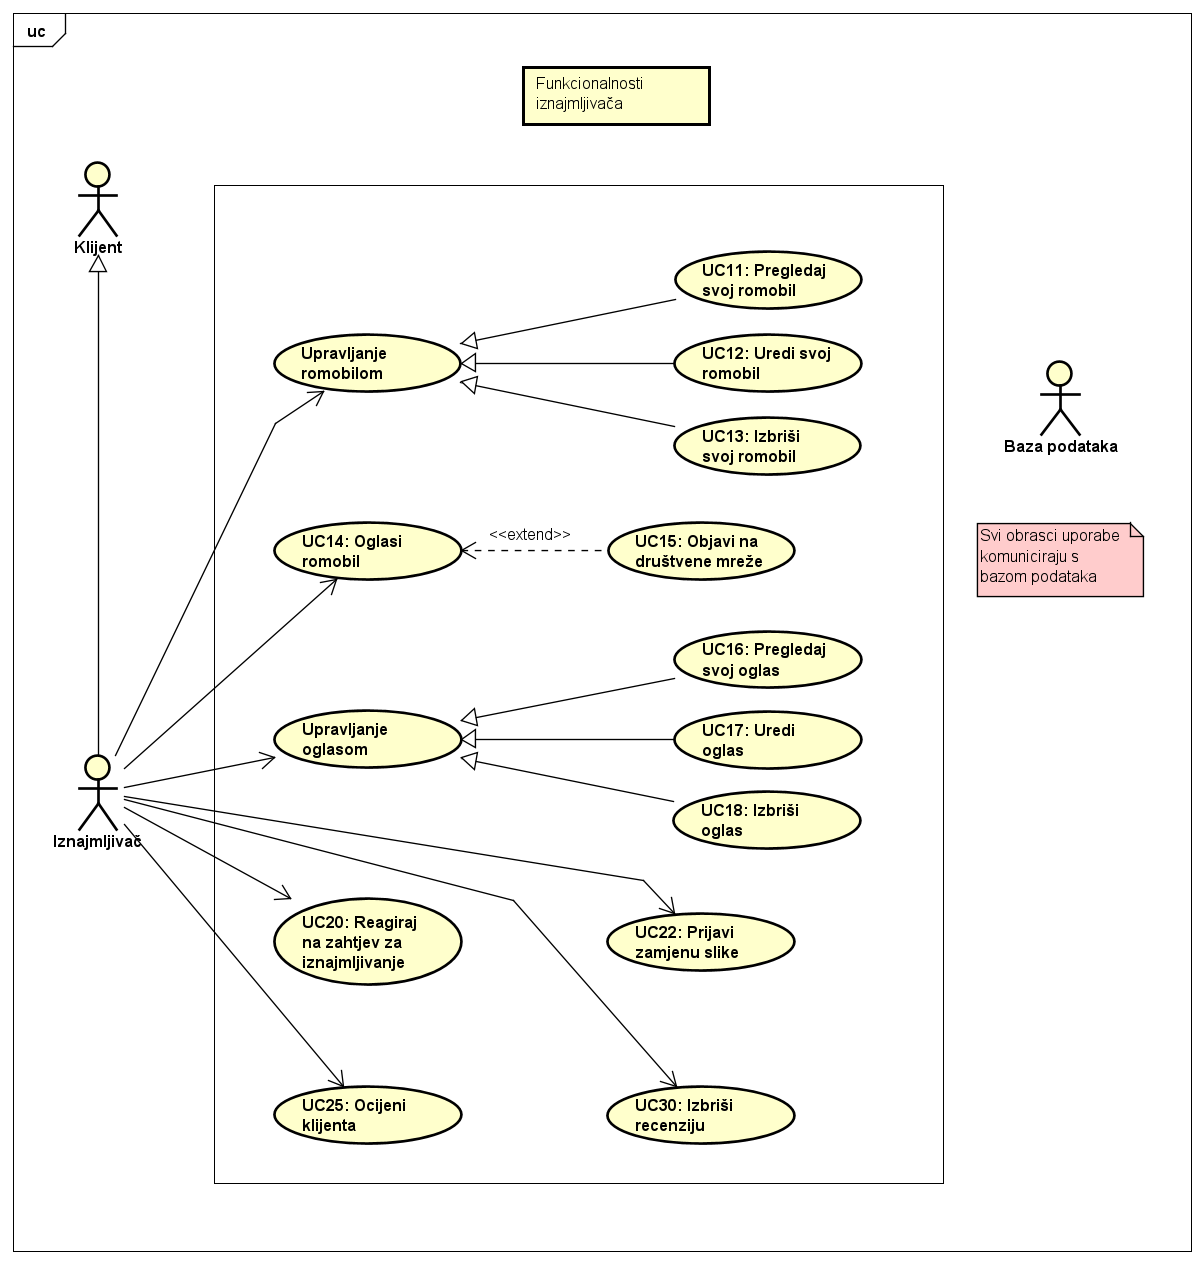
\includegraphics[width=1\linewidth]{dijagrami/iznajmljivac.png}
						\centering
						\caption{Dijagram obrasca uporabe - funkcionalnost iznajmljivača}
						\label{fig:Dijagram obrasca uporabe - funkcionalnost iznajmljivača}
					\end{figure}
					
					\begin{figure} [H]
						
						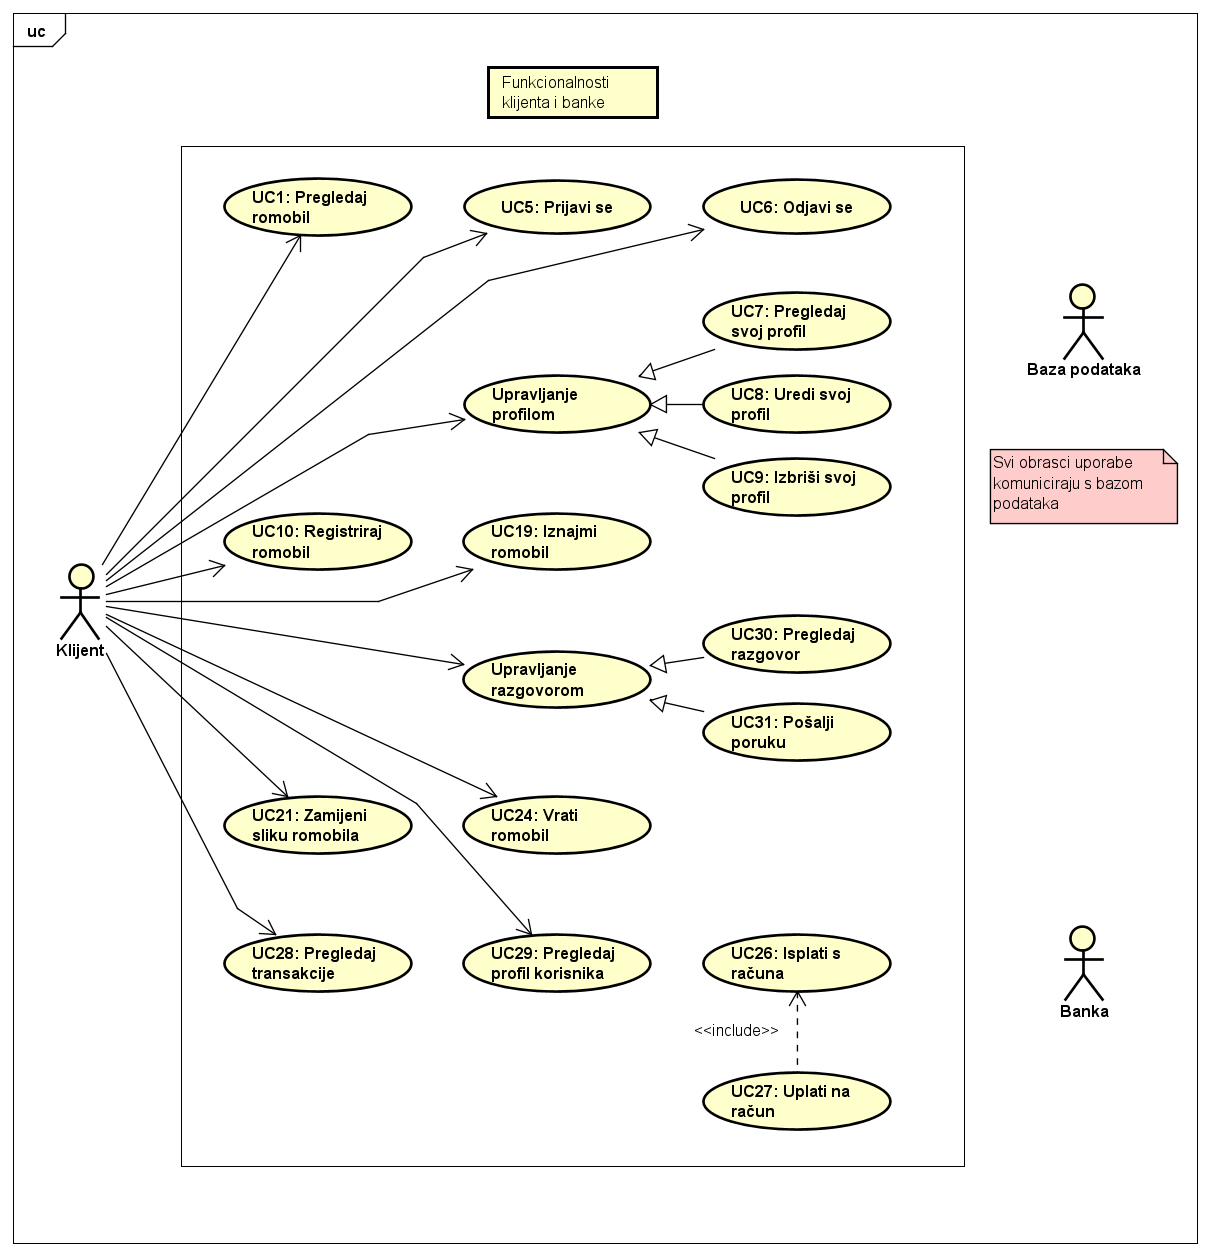
\includegraphics[width=1\linewidth]{dijagrami/klijent.png}
						\centering
						\caption{Dijagram obrasca uporabe - funkcionalnost klijenta i banke}
						\label{fig:Dijagram obrasca uporabe - funkcionalnost klijenta i banke}
					\end{figure}
					
					\begin{figure} [H]
						
						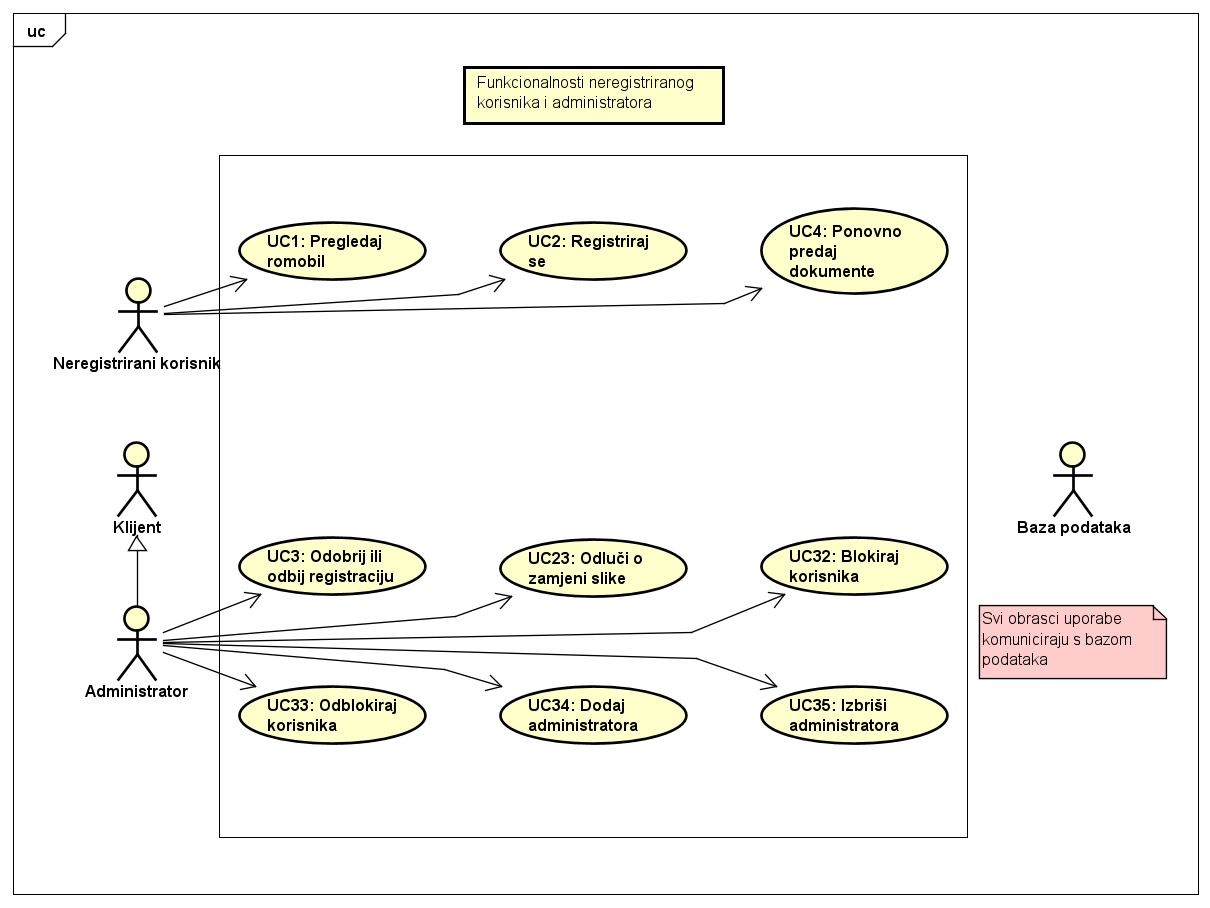
\includegraphics[width=1\linewidth]{dijagrami/admin_neregistrirani.png}
						\centering
						\caption{Dijagram obrasca uporabe - funkcionalnost neregistriranog korisnika i administratora}
						\label{fig:Dijagram obrasca uporabe - funkcionalnost neregistriranog korisnika i administratora}
					\end{figure}
					
					
					
				\eject		
				
			\subsection{Sekvencijski dijagrami}

				\subsubsection{Obrazac uporabe UC10 - Registriraj romobil}
						Klijent šalje zahtjev za prikaz stranice s njegovim registriranim romobilima. Poslužitelj iz baze dohvaća registrirane romobile tog klijenta. Ako klijent ima već registrirane romobile, poslužitelj ih prikazuje, inače poslužitelj prikazuje klijentu poruku da nema registriranih romobila. Klijent započinje registraciju romobila tako što zatraži od poslužitelja da mu prikaže obrazac za registraciju. Poslužitelj mu prikazuje prazan obrazac i klijent unosi podatke za registraciju te ih vraća poslužitelju. Poslužitelj provjerava jesu li podatci ispravno uneseni. Sve dok klijent ne unese ispravne podatke ispisuje mu se poruka da su podatci neispravni, unosi nove podatke koje zatim provjerava poslužitelj i vraća informaciju jesu li podatci ispravni ili ne. Kada klijent unese ispravne podatke za registraciju, potvrđuje svoj unos i poslužitelj te podatke prosljeđuje bazi koja pohranjuje registraciju. Romobil se nakon registracije prikazuje među klijentovim registriranim romobilima. Ako klijent do sada nije imao ulogu iznajmljivača, sada mu se dodjeljuje. 
						
						\begin{figure} [H]
							
							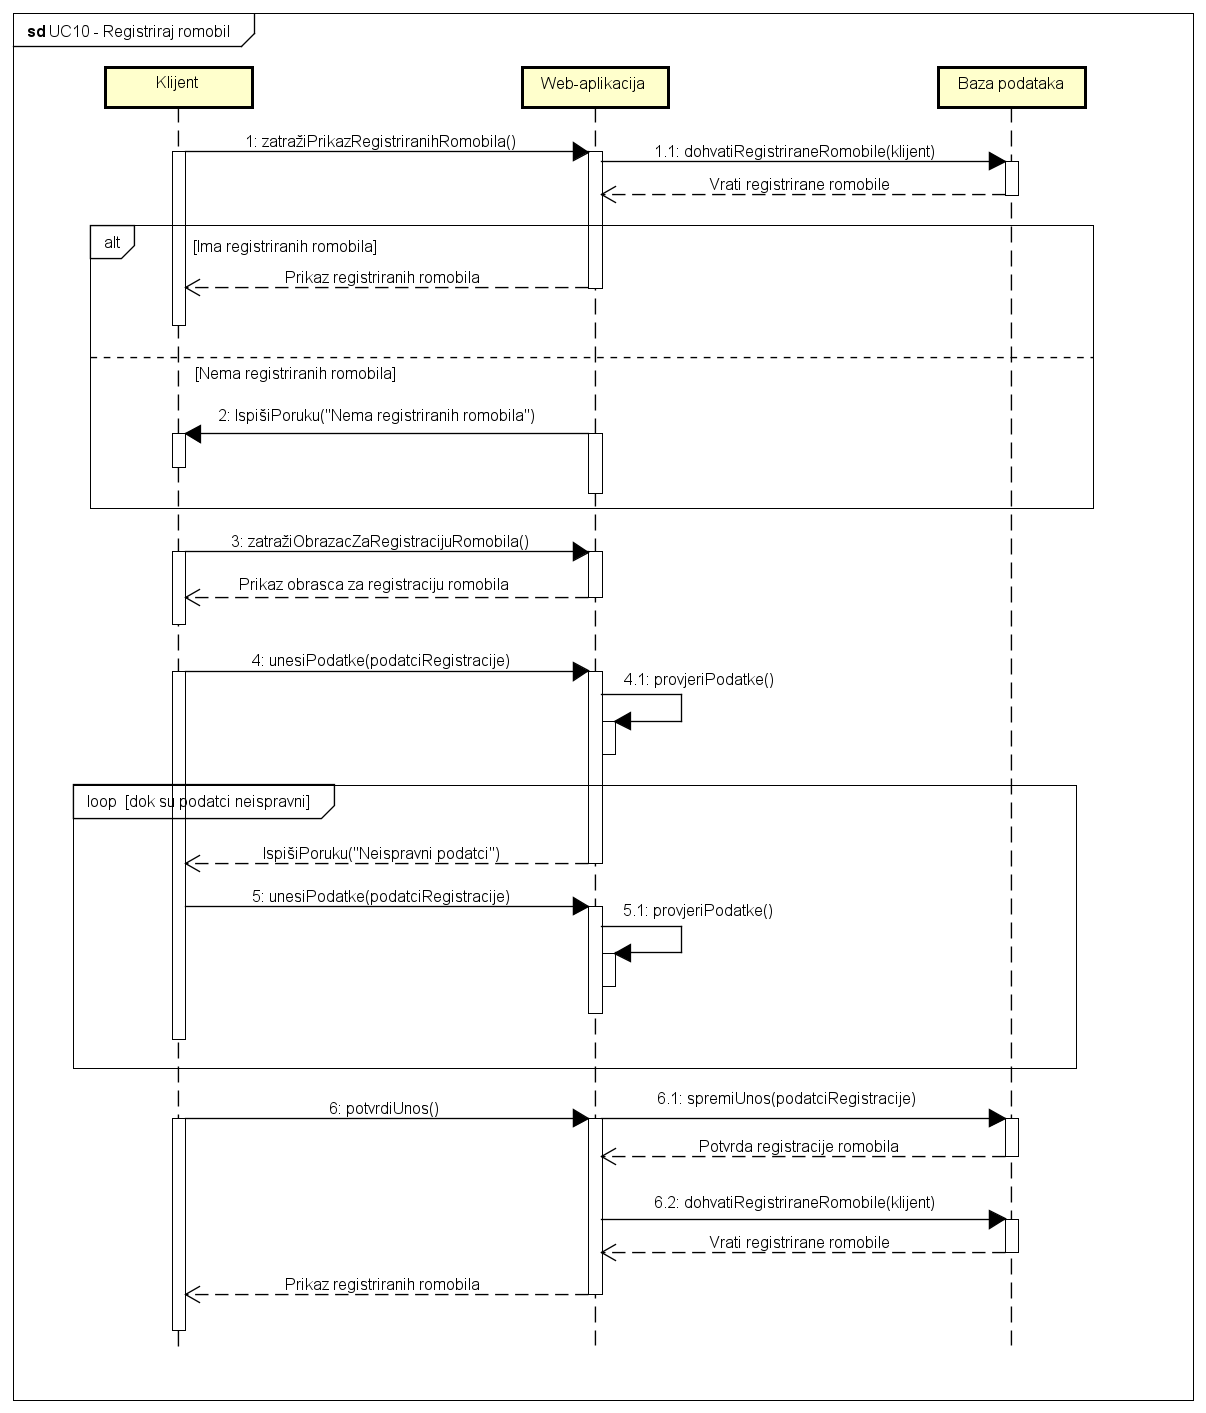
\includegraphics[width=1\linewidth]{dijagrami/UC10 - Registriraj romobil.png}
							\centering
							\caption{Sekvencijski dijagram obrasca UC10 - Registriraj romobil}
							\label{fig:Sekvencijski dijagram obrasca UC10 - Registriraj romobil}
						\end{figure}
				
				\eject

				\subsubsection{Obrazac uporabe UC14 - Oglasi romobil}
						Iznajmljivač šalje zahtjev za prikaz stranice s njegovim registriranim romobilima. Poslužitelj iz baze dohvaća registrirane romobile tog iznajmljivača i prikazuje mu ih. Iznajmljivač započinje stvaranje oglasa tako što zatraži da mu poslužitelj pošalje obrazac koji mora ispuniti. Poslužitelj prikazuje iznajmljivaču obrazac i iznajmljivač unosi podatke o oglasu te ih vraća poslužitelju. Poslužitelj provjerava jesu li podatci ispravno uneseni. Sve dok iznajmljivač ne unese ispravne podatke ispisuje mu se poruka da su podatci neispravni, unosi nove podatke koje zatim provjerava poslužitelj i vraća informaciju jesu li podatci ispravni ili ne. Kada iznajmljivač unese ispravne podatke za registraciju, potvrđuje svoj unos i poslužitelj te podatke prosljeđuje bazi koja pohranjuje oglas. Iznajmljivač dobiva poruku da je oglas uspješno postavljen. Oglas se prikazuje među oglasima dostupnim za iznajmljivanje.
						
						\begin{figure} [H]
							
							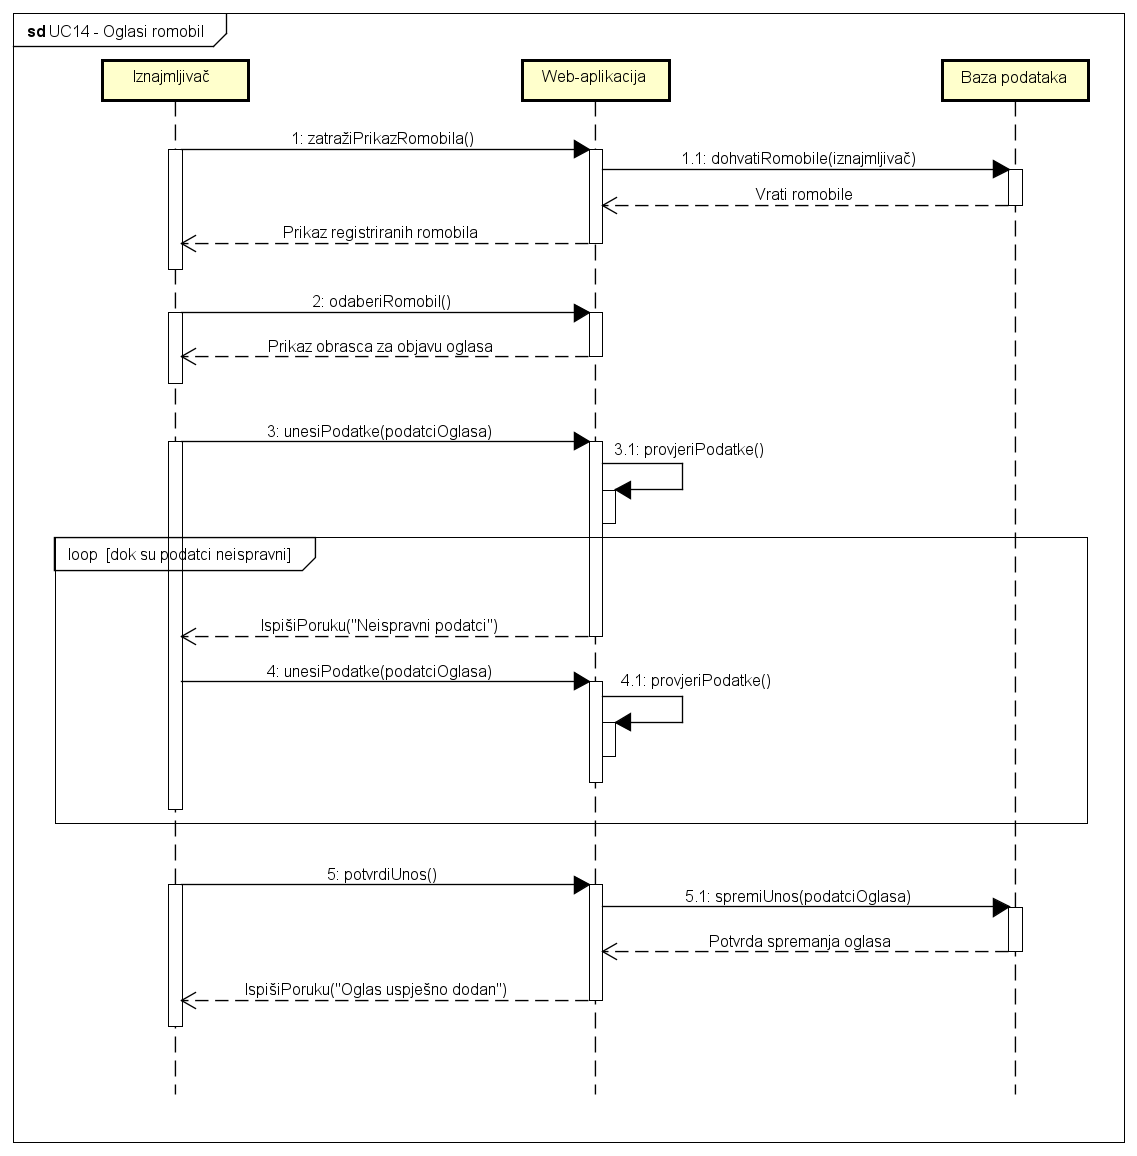
\includegraphics[width=1\linewidth]{dijagrami/UC14 - Oglasi romobil.png}
							\centering
							\caption{Sekvencijski dijagram obrasca UC14 - Oglasi romobil}
							\label{fig:Sekvencijski dijagram obrasca UC14 - Oglasi romobil}
						\end{figure}
						
				\eject

				\subsubsection{Obrazac uporabe UC20 - Reagiraj na zahtjev za iznajmljivanje}
				Iznajmljivač inicira zahtjev za pregled trenutačnih zahtjeva za najam kako bi odgovorio na klijentovu želju za najmom romobila. Poslužitelj preuzima trenutne zahtjeve koje je iznajmljivač poslao i prikazuje ih. Iznajmljivač zatim donosi odluku o prihvaćanju ili odbijanju zahtjeva, a svoj odabir označava u aplikaciji. Poslužitelj prosljeđuje tu informaciju bazi podataka kako bi se ažurirao status zahtjeva. U slučaju prihvaćanja zahtjeva za najam, oglas za najam romobila se uklanja iz baze podataka, a informacija o nedostupnosti romobila se pohranjuje. Nakon što se promjene spreme u bazu podataka, sustav obavještava klijenta o odluci iznajmljivača putem aplikacijske obavijesti.
				
				\begin{figure} [H]
					
					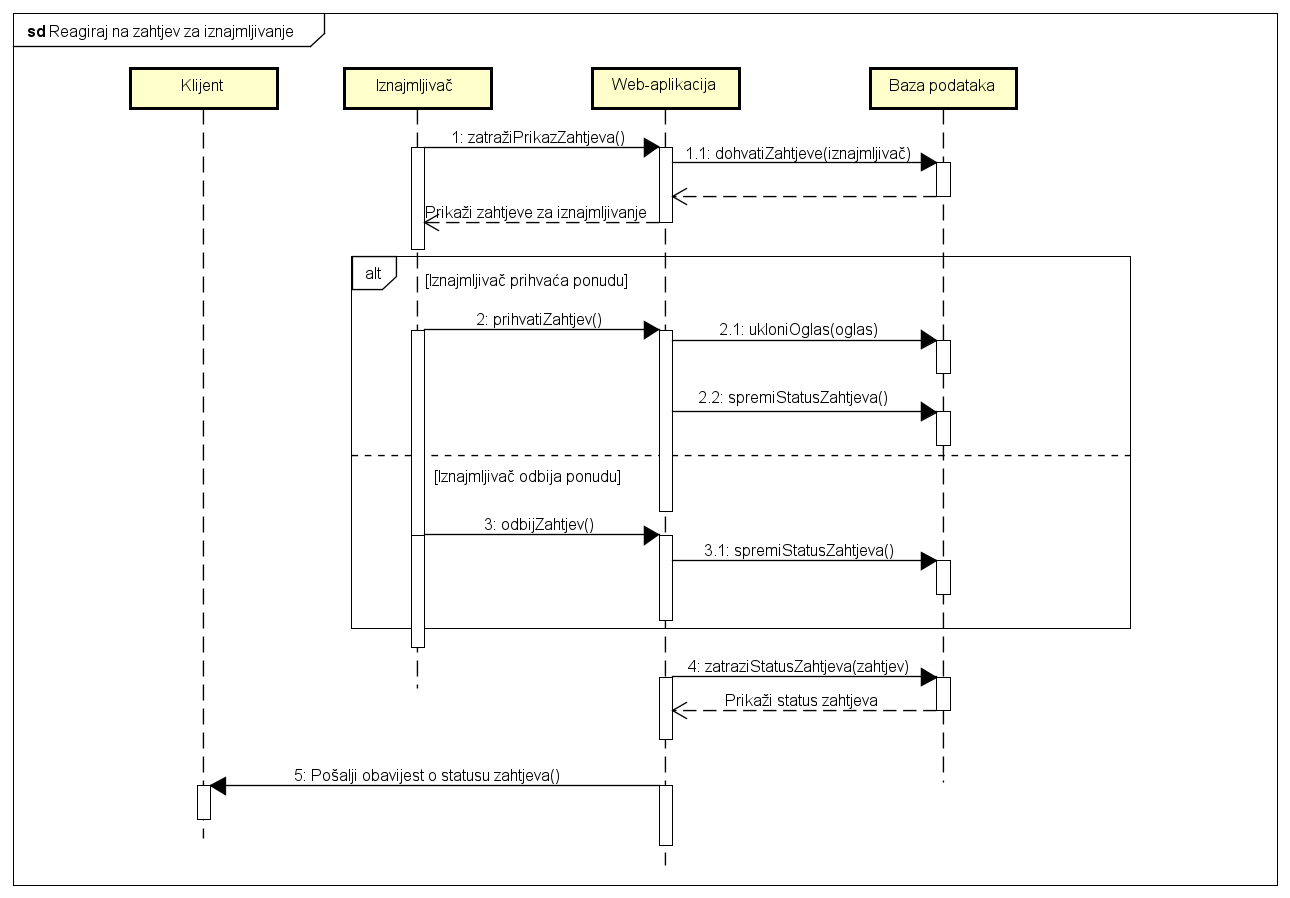
\includegraphics[width=1\linewidth]{dijagrami/UC20 - Reagiraj na zahtjev za iznajmljivanje.png}
					\centering
					\caption{Sekvencijski dijagram obrasca UC20 - Reagiraj na zahtjev za iznajmljivanje}
					\label{fig:Sekvencijski dijagram obrasca UC20 - Reagiraj na zahtjev za iznajmljivanje}
				\end{figure}
				
				\eject

				\subsubsection{Obrazac uporabe UC24 - Vrati romobil}
						Pri povratku romobila na kraju iznajmljivanja klijent zatraži od poslužitelja sve svoje aktivne najmove. Baza podataka pronalazi aktivne najmove tog klijenta i vraća ih poslužitelju. Ako klijent nema nijedan aktivan najam poslužitelj mu vraća poruku koja ga o tome obavještava. U slučaju da aktivni najmovi postoje, poslužitelj ih vraća klijentu. Klijent odabire za koji romobil želi potvrditi da je vraćen i šalje poslužitelju zahtjev da završi iznajmljivanje. Poslužitelj zabilježava kraj u bazi podataka i izračunava broj prijeđenih kilometara i cijenu najma. Informacije o transakciji za taj najam spremaju se u bazu podataka. Poslužitelj prikazujje obavijest o cijeni najma iznajmljivaču i klijentu koji su u najmu sudjelovali.
						
						\begin{figure} [H]
							
							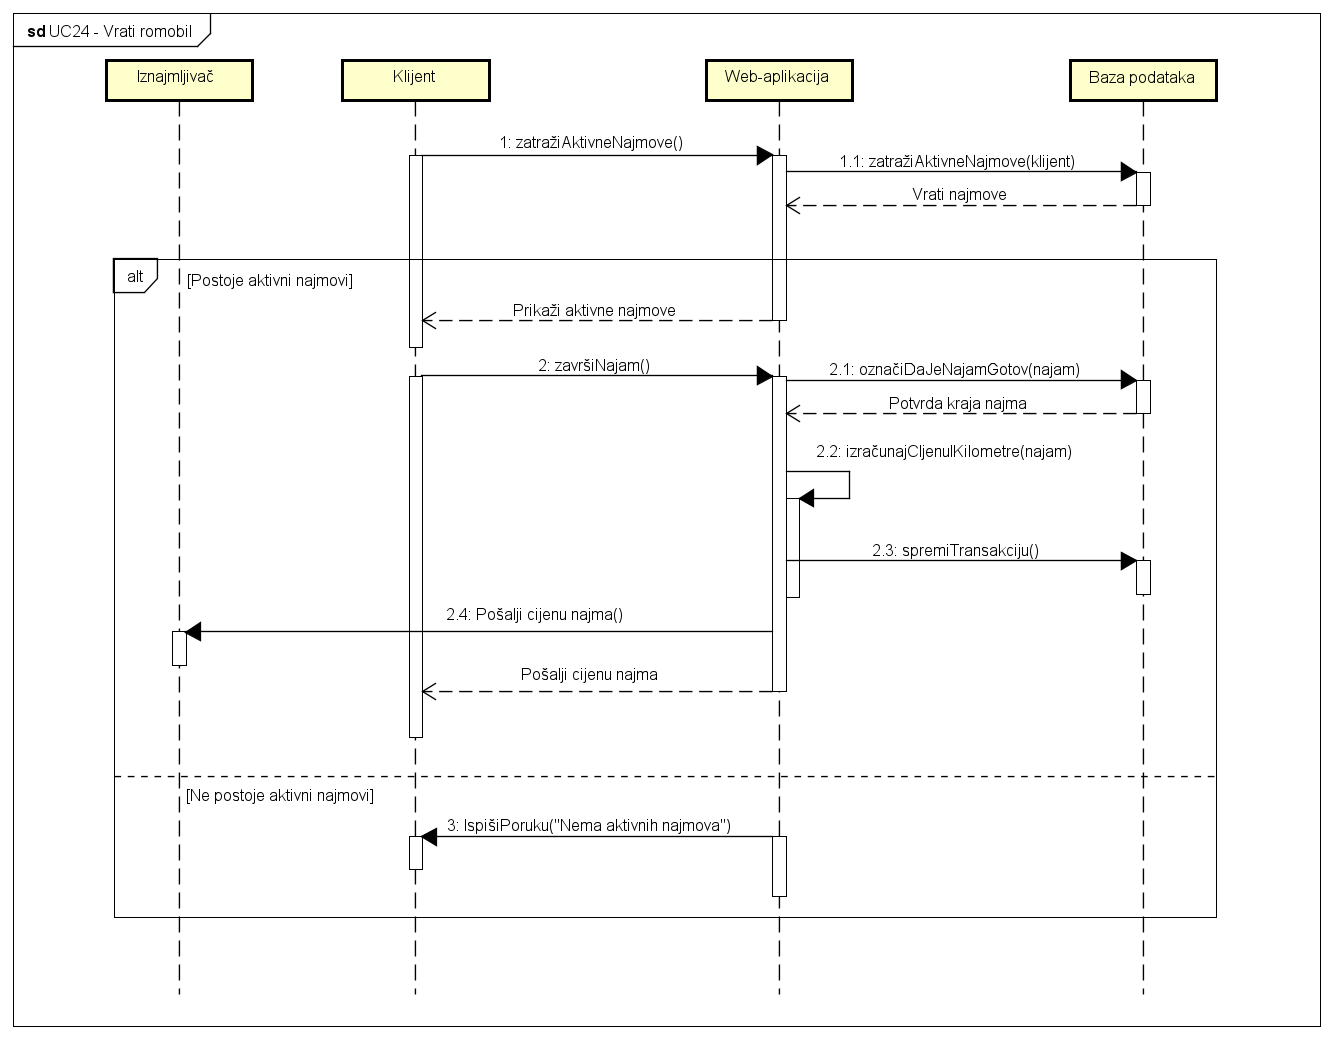
\includegraphics[width=1\linewidth]{dijagrami/UC24 - Vrati romobil.png}
							\centering
							\caption{Sekvencijski dijagram obrasca UC24 - Vrati romobil}
							\label{fig:Sekvencijski dijagram obrasca UC24 - Vrati romobil}
						\end{figure}
				\eject
	

		\section{Ostali zahtjevi}
		
			
		 
			 \begin{packed_item}
			 	\item Aplikacija mora se moći pokrenuti na svakome web-pregledniku
			 	\item Aplikacija mora biti javno dostupna
			 	\item Sustav mora omogućiti rad više korisnika u stvarnom vremenu
			 	\item Korisničko sučelje i sustav moraju podržavati hrvatsku abecedu (dijakritičke znakove)
			 	\item Neispravno korištenje korisničkog sučelja ne smije narušiti funkcionalnost i rad sustava
			 	\item Službena valuta sustavu je EURO (€)
			 	\item Sustav treba biti jednostavan za korištenje
			 	\item Sustav mora biti ostvaren koristeći objektno orijentirane jezike
			 	
			 	
			 \end{packed_item}
			 
			 
			 
	
	\chapter{Arhitektura i dizajn sustava}

\subsection{Opis arhitekture}

\textit{Detaljnom razradom cilja projektnog zadatka, u kojem je fokus izrada aplikacije za iznajmljivanje električnih romobila, definirali smo razinu klijenta, razinu web-aplikacije te sloj pristupa podatcima kao osnovne razine naše aplikacije.}

\subsubsection{Razina klijenta}

\textit{Razina klijenta predstavlja korisničko sučelje web-aplikacije koje korisnici vide i s kojim interagiraju. U razvoju projekta korišten je React, odnosno JavaScript knjižica za izradu korisničkog sučelja. Organizirano je u komponente koje predstavljaju određene dijelove korisničkog sučelja. Korišten je virtualni DOM (Document Object Model), kojim se ubrzava proces ažuriranja promjena korisničkog sučelja u svrhu poboljšavanja performansi web-aplikacije. }
\subsubsection{Razina web-aplikacije}

\textit{Sloj web-aplikacije je odgovoran za obradu zahtjeva korisnika, poslovnu logiku i komunikaciju s bazom podataka. U razvoju projekta korišten je okvir za razvoj web aplikacija Spring Boot u programskom jeziku Java. U Spring Bootu, kontroleri su odgovorni za obradu HTTP zahtjeva i usmjeravanje na odgovarajuće servise za obradu zahtjeva. Obradu podataka, validaciju te logiku obavljaju servisi, dok modeli predstavljaju strukturu podataka koja se koristi za komunkaciju s bazom podataka te prenošenje podataka između kontrolera i servisa.}
\subsubsection{Sloj pristupa podatcima}

\textit{Sloj pristupa podacima je odgovoran za komunikaciju s bazom podataka i pristupanje podacima. Građen je od entiteta s vlastitim atributima koji predstavljaju modele podataka koji odgovaraju tablicama u bazi podataka.}

\textit{Sinteza ovih slojeva - korisničkog sučelja na razini Reacta, web-aplikacijskog sloja u Spring Bootu i sloja pristupa podacima u Spring Bootu - stvara temelj za razvoj visoko skalabilnih i funkcionalnih web-aplikacija. Korisnici ostvaruju interakciju s aplikacijom preko intuitivnog React korisničkog sučelja, dok Spring Boot preuzima odgovornost za obradu njihovih zahtjeva i poslovne logike. Istovremeno, sloj pristupa podacima omogućuje efikasnu komunikaciju s bazom podataka, omogućujući pohranu i dohvat podataka s pouzdanošću i učinkovitošću.}

\subsection{MVC arhitektura}
\textit{Model-View-Controller (MVC) je arhitekturni obrazac koji se koristi za organizaciju komponenti u softverskim aplikacijama, posebno u razvoju web-aplikacija. Osnovna svrha MVC-a je odvajanje različitih aspekata aplikacije kako bi se omogućila bolja organizacija, održavanje i skalabilnost. Sastoji se od tri glavne komponente:}
\begin{itemize}
	\item\textit{Model - predstavlja sloj koji je odgovoran za obradu podataka i poslovnu logiku aplikacije te sadrži podatke i pravila za njihovu obradu.}
	\item\textit{View - predstavlja sloj koji se odnosi na korisničko sučelje aplikacije i odgovoran je za prikazivanje podataka korisnicima. Ne obavlja nikakvu poslovnu logiku, samo prikazuje podatke koji mu se dostave iz modela.}
	\item\textit{Kontroler - posrednik između Model i View komponenti. Prima korisničke zahtjeve, obrađuje ih te komunicira s Modelom radi dohvaćanja ili ažuriranja podataka. Također, odlučuje koji View treba biti prikazan korisniku na temelju podataka iz Modela te korisničkih zahtjeva, upravlja tokom aplikacije te sadrži logiku za validaciju, autorizaciju i upravljanje sesijama.}
\end{itemize}

\textit{MVC arhitektura omogućuje precizno razgraničenje odgovornosti unutar aplikacije. Ovo strukturalno odvajanje olakšava razvoj aplikacije, čini ju lakšom za održavanje i omogućava efikasnije testiranje. Svaka od tri glavne komponente - Model, View i Controller - može se ponovno koristiti na različitim dijelovima aplikacije. To potiče efikasnost razvoja jer se već razvijeni dijelovi aplikacije mogu lako iskoristiti u drugim kontekstima. MVC omogućuje skalabilnost aplikacije jer se jasno razdvajaju različiti aspekti. Novi dijelovi funkcionalnosti mogu se dodavati bez narušavanja postojeće arhitekture, što omogućava aplikaciji da raste i prilagodi se promjenama. }


\section{Baza podataka}

\textit{U kontekstu našeg sustava, baza podataka igra ključnu ulogu, pružajući strukturiranu platformu za modeliranje stvarnog svijeta. Temeljni građevni blok ove baze je relacija, odnosno tablica koja je jasno definirana svojim imenom i skupom atributa. Glavna svrha baze podataka je olakšati brzu i jednostavnu pohranu, promjenu te izvlačenje podataka kako bi se omogućila daljnja analiza i obrada. Unutar baze podataka za našu aplikaciju, identificiramo nekoliko ključnih entiteta:
	\begin{itemize}
		\item 	\textit{User}
		\item 	\textit{Preferences}
		\item 	\textit{SocialMedia}
		\item 	\textit{PrivacySettings}
		\item 	\textit{Document}
		\item 	\textit{Scooter}
		\item 	\textit{Listing}
		\item 	\textit{Review}
		\item 	\textit{Transaction}
		\item 	\textit{Invoice}
		\item 	\textit{Notification}
		\item 	\textit{ChatSession}
		\item 	\textit{Message}
		\item 	\textit{ImageChangeRequest}
	\end{itemize}
}

\subsection{User}


\textit{Ovaj entitet sadrzava sve važne informacije o korisniku aplikacije. Sadrži atribute: userId, nickname, firstName, lastName, cardNumber, email, phoneNumber, password, role te status. Ovaj entitet ima One-to-one vezu s entitetom Preferences preko atributa userId, One-to-one vezu s entitetom PrivacySettings preko atributa userId, One-to-one vezu s entitetom SocialMedia preko atributa userId, One-to-one vezu s entitetom Document preko atributa userId, One-to-many vezu s entitetom Scooter preko atributa userId, One-to-many vezu s entitetom Listing preko atributa renterUsername, One-to-one vezu s entitetom Review preko atributa reviewerUsername, One-to-one vezu s entitetom Review preko atributa renterUsername, One-to-many vezu s entitetom ChatSessions preko atributa user1 ili atributa user2, Many-to-one vezu s entitetom Messages preko atributa senderUsername, One-to-many vezu s entitetom ImageChangeRequest preko atributa requesterId te One-to-many vezu s entitetom Notification preko atributa userId, requestingUser te decisionAdmin.}


\begin{longtblr}[
	label=none,
	entry=none
]{
	width = \textwidth,
	colspec={|X[6,l]|X[6, l]|X[20, l]|},
	rowhead = 1,
} %definicija širine tablice, širine stupaca, poravnanje i broja redaka naslova tablice
	\hline \SetCell[c=3]{c}{\textbf{User}}	 \\ \hline[3pt]
	\SetCell{LightGreen}userId & INT	&  jedinstveni identifikator korisnika	\\ \hline
	nickname	& VARCHAR &  jedinstveni nadimak korisnika  	\\ \hline
	firstName & VARCHAR &  ime korisnika  \\ \hline
	lastName & VARCHAR	& prezime korisnika
	\\ \hline
	cardNumber	& INT &   broj kartice korisnika	\\ \hline
	email	& VARCHAR &    jedinstvena email adresa korisnika	\\ \hline
	phoneNumber	& INT &   jedinstveni kontakt broj korisnika 	\\ \hline
	password	& VARCHAR & zaporka za prijavu korisnika   	\\ \hline
	role	& UserRole &  uloga korisnika (unregistered, registered, renter, admin) 	\\ \hline
	status	& UserStatus & status korisnika (pending, rejected, accepted, blocked) 	\\ \hline
\end{longtblr}

\subsection{Preferences}


\textit{Ovaj entitet sadrzava sve važne informacije o preferencama korisnika aplikacije. Sadrži atribute: userId, language i darkMode. Ovaj entitet ima One-to-one vezu s entitetom User preko atributa userId.}


\begin{longtblr}[
	label=none,
	entry=none
]{
	width = \textwidth,
	colspec={|X[6,l]|X[6, l]|X[20, l]|},
	rowhead = 1,
} %definicija širine tablice, širine stupaca, poravnanje i broja redaka naslova tablice
	\hline \SetCell[c=3]{c}{\textbf{Preferences}}	 \\ \hline[3pt]
	\SetCell{LightGreen}userId & INT	&  jedinstveni identifikator korisnika	 	\\ \hline
	language	& UserLanguage & jezik korisnika   	\\ \hline
	darkMode & BOOLEAN &  omogućen dark mode \\ \hline
\end{longtblr}

\subsection{Social Media}


\textit{Ovaj entitet sadrzava sve važne informacije o socijalnim mrežama korisnika aplikacije. Sadrži atribute: userId, instagram, facebook, google i tikTok. Ovaj entitet ima One-to-one vezu s entitetom User preko atributa userId.}


\begin{longtblr}[
	label=none,
	entry=none
]{
	width = \textwidth,
	colspec={|X[6,l]|X[6, l]|X[20, l]|},
	rowhead = 1,
} %definicija širine tablice, širine stupaca, poravnanje i broja redaka naslova tablice
	\hline \SetCell[c=3]{c}{\textbf{Social Media}}	 \\ \hline[3pt]
	\SetCell{LightGreen}userId & INT	&  jedinstveni identifikator korisnika	 	\\ \hline
	instagram	& VARCHAR &   	instagram account korisnika \\ \hline
	facebook & VARCHAR & facebook account korisnika  \\ \hline
	google & VARCHAR	&  google account korisnika		\\ \hline
	tikTok	& VARCHAR &  tikTok account korisnika 	\\ \hline
\end{longtblr}

\subsection{PrivacySettings}


\textit{Ovaj entitet sadrzava sve važne informacije o postavkama privatnosti korisnika aplikacije. Sadrži atribute: userId, isFirstNameVisible, isLastNameVisible, isNicknameVisible i isEmailVisible. Ovaj entitet ima One-to-one vezu s entitetom User preko atributa userId.}


\begin{longtblr}[
	label=none,
	entry=none
]{
	width = \textwidth,
	colspec={|X[6,l]|X[6, l]|X[20, l]|},
	rowhead = 1,
} %definicija širine tablice, širine stupaca, poravnanje i broja redaka naslova tablice
	\hline \SetCell[c=3]{c}{\textbf{Privacy Settings}}	 \\ \hline[3pt]
	\SetCell{LightGreen}userId & INT	&  	 jedinstveni identifikator korisnika	\\ \hline
	isFirstNameVisible	& BOOLEAN &   omogućena vidljivost imena korisnika	\\ \hline
	isLastNameVisible & BOOLEAN &   omogućena vidljivost prezimena korisnika\\ \hline
	isNicknameVisible & BOOLEAN	&  		omogućena vidljivost nadimka korisnika\\ \hline
	isEmailVisible & BOOLEAN	&  		omogućena vidljivost emaila korisnika\\ \hline
\end{longtblr}

\subsection{Document}


\textit{Ovaj entitet sadrzava sve važne informacije o dokumentima korisnika aplikacije. Sadrži atribute: userId, criminalRecordURL, identificationDocumentURL i status. Ovaj entitet ima One-to-one vezu s entitetom User preko atributa userId.}


\begin{longtblr}[
	label=none,
	entry=none
]{
	width = \textwidth,
	colspec={|X[6,l]|X[6, l]|X[20, l]|},
	rowhead = 1,
} %definicija širine tablice, širine stupaca, poravnanje i broja redaka naslova tablice
	\hline \SetCell[c=3]{c}{\textbf{Document}}	 \\ \hline[3pt]
	\SetCell{LightGreen}userId & INT	&  jedinstveni identifikator korisnika	 	\\ \hline
	criminalRecordURL	& VARCHAR &  url kaznene evidencije	\\ \hline
	identificationDocumentURL & VARCHAR &  url identifikacijskog dokumenta \\ \hline
	status & DocumentStatus	& status dokumenta (pending, approved, rejected) 		\\ \hline
\end{longtblr}

\subsection{Scooter}


\textit{Ovaj entitet sadrzava sve važne informacije o pojedinom romobilu. Sadrži atribute:scooterId, manufacturer, model, batteryCapacity, maxSpeed, imageUrl, maxRange, yearOfManufacture, additionalInformation, userId i availability. Ovaj entitet ima Many-to-one vezu s entitetom User preko atributa userId te One-to-many vezu s entitetom Listings preko atributa scooterId.}


\begin{longtblr}[
	label=none,
	entry=none
]{
	width = \textwidth,
	colspec={|X[6,l]|X[6, l]|X[20, l]|},
	rowhead = 1,
} %definicija širine tablice, širine stupaca, poravnanje i broja redaka naslova tablice
	\hline \SetCell[c=3]{c}{\textbf{Scooter}}	 \\ \hline[3pt]
	\SetCell{LightGreen}scooterId & INT	&  	jedinstveni identifikator romobila 	\\ \hline
	manufacturer	& VARCHAR & proizvođač romobila  	\\ \hline
	model & VARCHAR &  model romobila \\ \hline
	batteryCapacity & INT	& kapacitet baterije 		\\ \hline
	maxSpeed 	& INT &   maksimalna brzina	\\ \hline
	imageUrl	& TEXT &  url slike 	\\ \hline
	maxRange	& FLOAT & maksimalni domet  	\\ \hline
	yearOfManufacture	& INT &   	godina proizvodnje\\ \hline
	additionalInformation	& TEXT &  dodatne informacije 	\\ \hline
	userId	& INT & jedinstveni identifikator korisnika  	\\ \hline
	\SetCell{LightBlue}availability	& BOOLEAN &  dostupnost 	\\ \hline
\end{longtblr}

\subsection{Listing}


\textit{Ovaj entitet sadrzava sve važne informacije o pojedinom oglasu. Sadrži atribute:listingId, currentAddress, returnAddress, returnByTime, pricePerKilometer, penaltyFee, scooterId, listingTime, notes i status. Ovaj entitet ima Many-to-one vezu s entitetom Scooter preko atributa scooterId te One-to-many vezu s entitetom Transactions preko atributa listingId.}


\begin{longtblr}[
	label=none,
	entry=none
]{
	width = \textwidth,
	colspec={|X[6,l]|X[6, l]|X[20, l]|},
	rowhead = 1,
} %definicija širine tablice, širine stupaca, poravnanje i broja redaka naslova tablice
	\hline \SetCell[c=3]{c}{\textbf{Listing}}	 \\ \hline[3pt]
	\SetCell{LightGreen}listingId & INT	&  jedinstveni identifikator oglasa	 	\\ \hline
	currentAddress	& VARCHAR & trenutna adresa  	\\ \hline
	returnAddress & VARCHAR	& adresa povratka 		\\ \hline
	returnByTime 	& TIMESTAMP & vrijeme vraćanja   	\\ \hline
	pricePerKilometer	& FLOAT &   cijena po kilometru	\\ \hline
	penaltyFee	& FLOAT &   	kaznena naknada\\ \hline
	\SetCell{LightBlue}scooterId	& INT &  jedinstveni identifikator romobila 	\\ \hline
	listingTime	& TIMESTAMP &   	vrijeme objave oglasa\\ \hline
	notes	& TEXT &  bilješke 	\\ \hline
	status	& ListingStatus &   	status oglasa (active, finished, cancelled)\\ \hline
\end{longtblr}

\subsection{Review}


\textit{Ovaj entitet sadrzava sve važne informacije o pojedinom osvrtu. Sadrži atribute: transactionId, reviewerUsername, renterUsername, stars, comment te reviewTime. Ovaj entitet ima Ona-to-one vezu s entitetom User preko atributa reviewerUsername, One-to-one vezu s entitetom User preko atributa renterUsername te One-to-one vezu s entitetom Transaction preko atributa transactionId.}


\begin{longtblr}[
	label=none,
	entry=none
]{
	width = \textwidth,
	colspec={|X[6,l]|X[6, l]|X[20, l]|},
	rowhead = 1,
} %definicija širine tablice, širine stupaca, poravnanje i broja redaka naslova tablice
	\hline \SetCell[c=3]{c}{\textbf{Review}}	 \\ \hline[3pt]
	\SetCell{LightGreen}transactionId & INT	&  jedinstveni identifikator transakcije	 	\\ \hline
	\SetCell{LightBlue}reviewerUsername	& VARCHAR &  korisničko ime recenzenta 	\\ \hline
	\SetCell{LightBlue}renterUsername & VARCHAR &  korisničko ime iznajmljivača \\ \hline
	stars & INT	&  	broj zvjezdica/ocjena	\\ \hline
	comment	& TEXT &  komentar 	\\ \hline
	reviewTime	& TIMESTAMP &   vrijeme osvrta	\\ \hline
\end{longtblr}

\subsection{Transaction}


\textit{Ovaj entitet sadrzava sve važne informacije o pojedinoj transakciji. Sadrži atribute: transactionId, kilometersTraveled, totalPrice, listingId, paymentTime te previousTransactionStatus. Ovaj entitet ima Many-to-one vezu s entitetom Listing preko atributa listingId te One-to-one vezu s entitetom Invoice preko atributa transactionId.}


\begin{longtblr}[
	label=none,
	entry=none
]{
	width = \textwidth,
	colspec={|X[6,l]|X[6, l]|X[20, l]|},
	rowhead = 1,
} %definicija širine tablice, širine stupaca, poravnanje i broja redaka naslova tablice
	\hline \SetCell[c=3]{c}{\textbf{Transaction}}	 \\ \hline[3pt]
	\SetCell{LightGreen}transactionId & INT	&  jedinstveni identifikator transakcije	 	\\ \hline
	kilometersTraveled	& FLOAT &   broj prijeđenih kilometara	\\ \hline
	totalPrice	& FLOAT &   ukupna cijena	\\ \hline
	\SetCell{LightBlue}listingId	& INT &   jedinstveni identifikator oglasa	\\ \hline
	paymentTime	& TIMESTAMP &   vrijeme plaćanja	\\ \hline
	transactionStatus	& TransactionStatus &   status transakcije	\\ \hline
\end{longtblr}

\subsection{Invoice}


\textit{Ovaj entitet sadrzava sve važne informacije o pojedinoj dostavnici. Sadrži atribute:transactionId, invoiceNumber te paymentMethod. Ovaj entitet ima One-to-one vezu s entitetom Transaction preko atributa transactionId.}


\begin{longtblr}[
	label=none,
	entry=none
]{
	width = \textwidth,
	colspec={|X[6,l]|X[6, l]|X[20, l]|},
	rowhead = 1,
} %definicija širine tablice, širine stupaca, poravnanje i broja redaka naslova tablice
	\hline \SetCell[c=3]{c}{\textbf{Invoice}}	 \\ \hline[3pt]
	\SetCell{LightGreen}transactionId  & INT	&  	 jedinstveni identifikator transakcije	\\ \hline
	invoiceNumber	& INT &   broj fakture	\\ \hline
	paymentMethod & PaymentMethod &   način plaćanja (PayPal, kekspay, Revolut)\\ \hline
\end{longtblr}

\subsection{Notification}


\textit{Ovaj entitet sadrzava sve važne informacije o pojedinoj obavijesti. Sadrži atribute: notificationId, userId, requestingUser, decisionAdmin, content, isRead te sentTime. Ovaj entitet ima Many-to-one vezu s entitetom User preko atributa userId, Many-to-one vezu s entitetom User preko atributa requestingUser te Many-to-one vezu s entitetom User preko atributa decisionAdmin.}


\begin{longtblr}[
	label=none,
	entry=none
]{
	width = \textwidth,
	colspec={|X[6,l]|X[6, l]|X[20, l]|},
	rowhead = 1,
} %definicija širine tablice, širine stupaca, poravnanje i broja redaka naslova tablice
	\hline \SetCell[c=3]{c}{\textbf{Notification}}	 \\ \hline[3pt]
	\SetCell{LightGreen}notificationId & INT	&  	jedinstveni identifikator obavijesti 	\\ \hline
	\SetCell{LightBlue}userId	& INT &   	jedinstveni identifikator korisnika	\\ \hline
	\SetCell{LightBlue}requestingUser & INT & korisnik koji zahtjeva  \\ \hline
	\SetCell{LightBlue}decisionAdmin & INT	&  	admin za odluku	\\ \hline
	content	& TEXT &  sadržaj 	\\ \hline
	isRead	& BOOLEAN &   pročitanost	\\ \hline
	sentTime	& TIMESTAMP &   vrijeme slanja	\\ \hline
\end{longtblr}

\subsection{ChatSession}


\textit{Ovaj entitet sadrzava sve važne informacije o pojedinom razgovoru. Sadrži atribute: chatId, user1, user2, startCommunicationTime te lastMessageTime. Ovaj entitet ima Many-to-one vezu s entitetom User preko atributa user1, Many-to-one vezu s entitetom User preko atributa user2 te One-to-many vezu s entitetom Messages preko atributa sessionId.}


\begin{longtblr}[
	label=none,
	entry=none
]{
	width = \textwidth,
	colspec={|X[6,l]|X[6, l]|X[20, l]|},
	rowhead = 1,
} %definicija širine tablice, širine stupaca, poravnanje i broja redaka naslova tablice
	\hline \SetCell[c=3]{c}{\textbf{ChatSession}}	 \\ \hline[3pt]
	\SetCell{LightGreen} chatId & INT	&  	jedinstveni identifikator razgovora 	\\ \hline
	\SetCell{LightBlue}user1	& INT &   korisnik 1	\\ \hline
	\SetCell{LightBlue}user2 & INT &  korisnik 2 \\ \hline
	startCommunicationTime 	& TIMESTAMP &   vrijeme početka komunikacije	\\ \hline
	lastMessageTime	& TIMESTAMP &   vrijeme zadnje poslane poruke	\\ \hline
\end{longtblr}

\subsection{Message}


\textit{Ovaj entitet sadrzava sve važne informacije o pojedinoj poruci. Sadrži atribute:messageId, senderUsername, sessionId, text, sentTime te status. Ovaj entitet ima One-to-many vezu s entitetom User preko atributa senderUsername te Many-to-one vezu s entitetom ChatSession preko atributa sessionId.}


\begin{longtblr}[
	label=none,
	entry=none
]{
	width = \textwidth,
	colspec={|X[6,l]|X[6, l]|X[20, l]|},
	rowhead = 1,
} %definicija širine tablice, širine stupaca, poravnanje i broja redaka naslova tablice
	\hline \SetCell[c=3]{c}{\textbf{Message}}	 \\ \hline[3pt]
	\SetCell{LightGreen}messageId & INT	&  	jedinstveni identifikator poruke 	\\ \hline
	\SetCell{LightBlue}senderUsername	& VARCHAR &   nadimak pošiljatelja	\\ \hline
	\SetCell{LightBlue}sessionId & INT &  jedinstveni identifikator razgovora \\ \hline
	text & TEXT	&  	tekst	\\ \hline
	sentTime 	& TIMESTAMP &   vrijeme slanja	\\ \hline
	status	& MessageStatus &   status poruke (read, unread)	\\ \hline
\end{longtblr}

\subsection{ImageChangeRequest}


\textit{Ovaj entitet sadrzava sve važne informacije o zahtjevu za promjenom slike. Sadrži atribute: imageId, requesterId, listingId, newImageUrl, complaintTime, additionalComments, status, approvalTime te rejectionReason. Ovaj entitet ima Many-to-one vezu s entitetom User preko atributa requesterId te Many-to-one vezu s entitetom Listing preko atributa listingId.}


\begin{longtblr}[
	label=none,
	entry=none
]{
	width = \textwidth,
	colspec={|X[6,l]|X[6, l]|X[20, l]|},
	rowhead = 1,
} %definicija širine tablice, širine stupaca, poravnanje i broja redaka naslova tablice
	\hline \SetCell[c=3]{c}{\textbf{ImageChangeRequest}}	 \\ \hline[3pt]
	\SetCell{LightGreen}imageId & INT	&  	jedinstveni identifikator slike 	\\ \hline
	\SetCell{LightBlue}requesterId	& INT &   jedinstveni identifikator pošiljatelja	\\ \hline
	\SetCell{LightBlue}listingId & INT &  jedinstveni identifikator oglasa \\ \hline
	newImageUrl & VARCHAR	&  	url nove slike	\\ \hline
	complaintTime 	& TIMESTAMP &   vrijeme žalbe	\\ \hline
	additionalComments	& TEXT &   dodatni komentari	\\ \hline
	status	& ImageChangeRequestStatu &  status zahtjeva (approved, rejected, pending)	\\ \hline
	approvalTime	& TIMESTAMP &   vrijeme odobrenja	\\ \hline
	rejectionReason	& TEXT &   razlog odbitka	\\ \hline
\end{longtblr}



\subsection{Dijagram baze podataka}
\begin{figure}
	\centering
	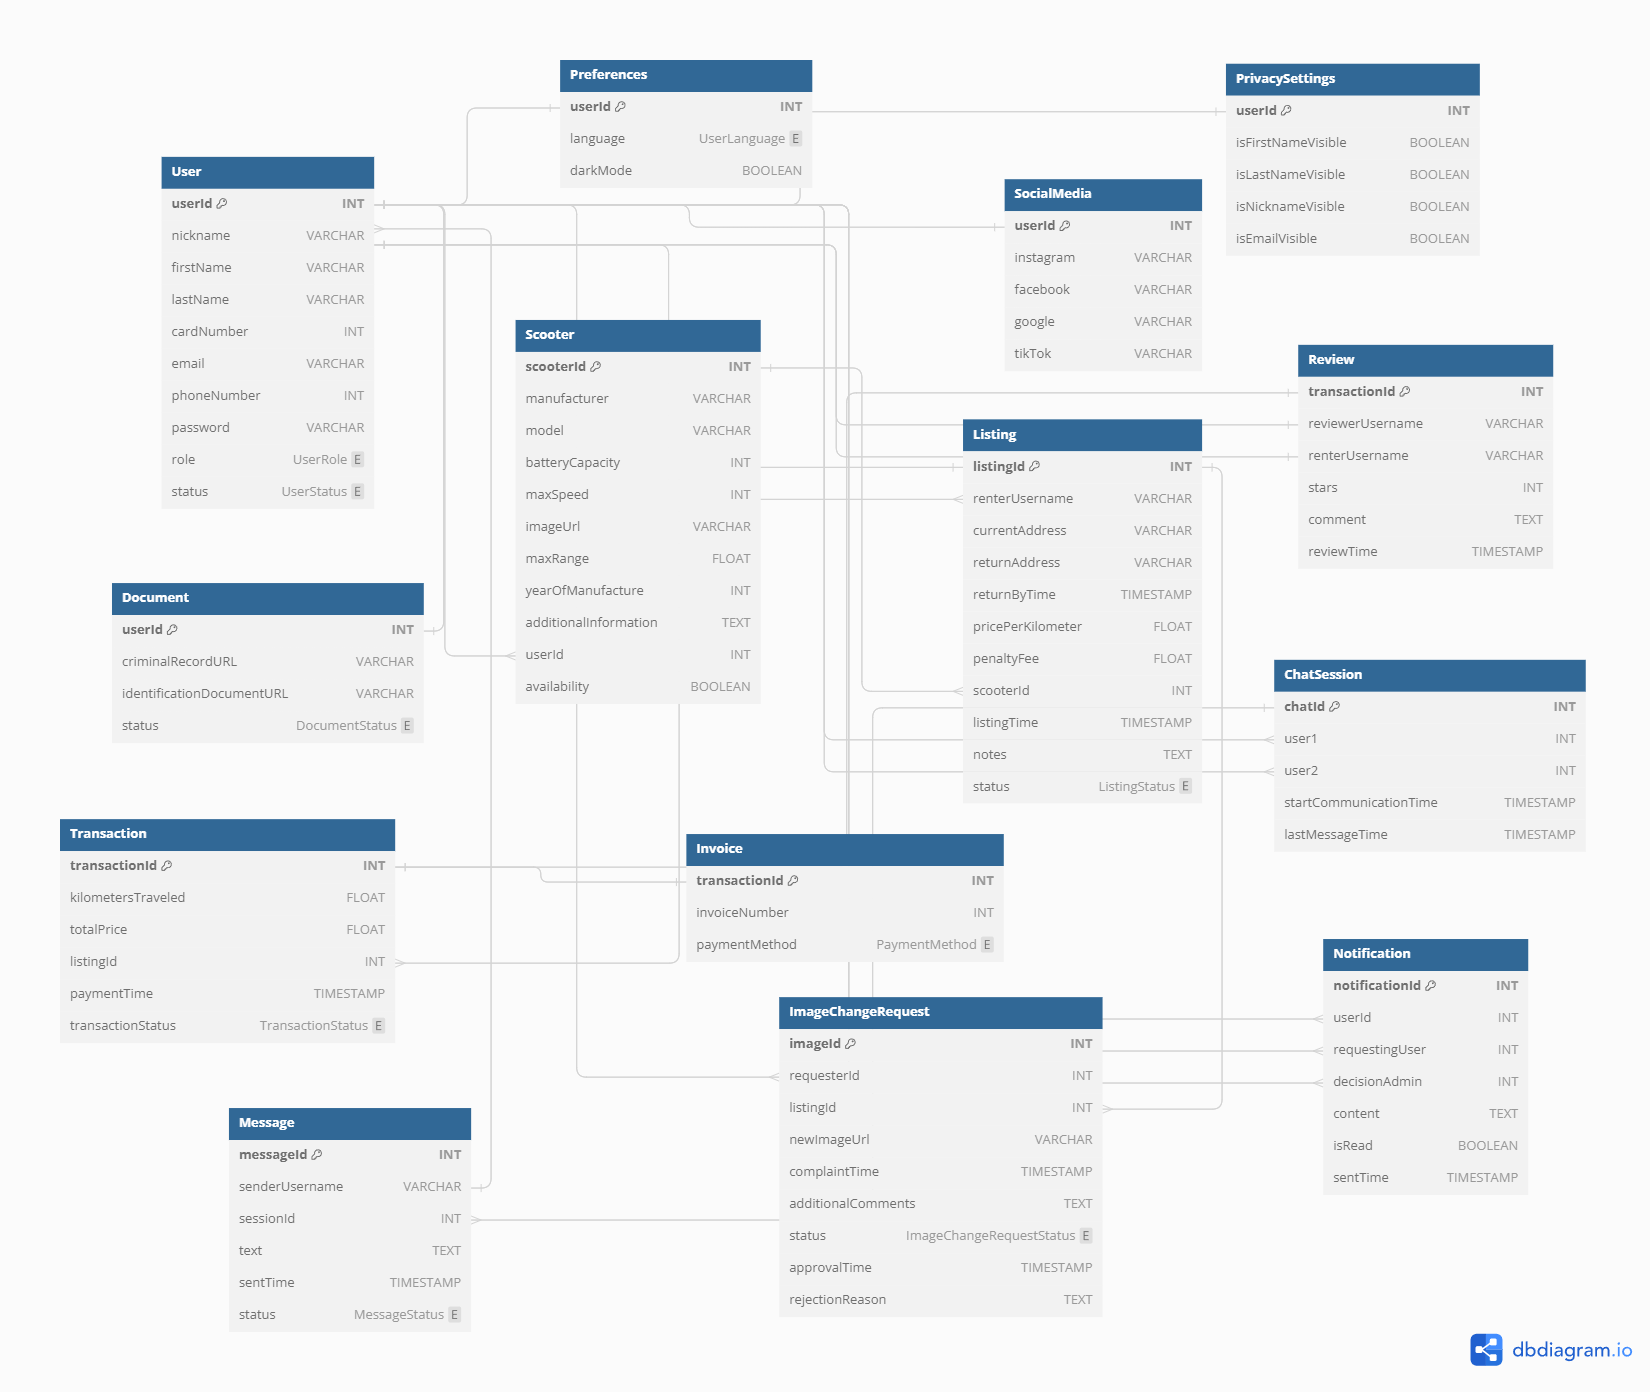
\includegraphics[width=0.5\linewidth]{slike/RelacijskiDijagramBP.png}
	\caption{Slika dijagrama baze podataka}
	\label{fig:Slika dijagrama baze podataka}
\end{figure}

	\chapter{Implementacija i korisničko sučelje}
		
		
		\section{Korištene tehnologije i alati}
		
			\textbf{\textit{dio 2. revizije}}
			
			 \textit{Detaljno navesti sve tehnologije i alate koji su primijenjeni pri izradi dokumentacije i aplikacije. Ukratko ih opisati, te navesti njihovo značenje i mjesto primjene. Za svaki navedeni alat i tehnologiju je potrebno \textbf{navesti internet poveznicu} gdje se mogu preuzeti ili više saznati o njima}.
			
			
			\eject 
		
	
		\section{Ispitivanje programskog rješenja}
			
			\textbf{\textit{dio 2. revizije}}\\
			
			 \textit{U ovom poglavlju je potrebno opisati provedbu ispitivanja implementiranih funkcionalnosti na razini komponenti i na razini cijelog sustava s prikazom odabranih ispitnih slučajeva. Studenti trebaju ispitati temeljnu funkcionalnost i rubne uvjete.}
	
			
			\subsection{Ispitivanje komponenti}
			\textit{Potrebno je provesti ispitivanje jedinica (engl. unit testing) nad razredima koji implementiraju temeljne funkcionalnosti. Razraditi \textbf{minimalno 6 ispitnih slučajeva} u kojima će se ispitati redovni slučajevi, rubni uvjeti te izazivanje pogreške (engl. exception throwing). Poželjno je stvoriti i ispitni slučaj koji koristi funkcionalnosti koje nisu implementirane. Potrebno je priložiti izvorni kôd svih ispitnih slučajeva te prikaz rezultata izvođenja ispita u razvojnom okruženju (prolaz/pad ispita). }
			
			
			
			\subsection{Ispitivanje sustava}
			
			 \textit{Potrebno je provesti i opisati ispitivanje sustava koristeći radni okvir Selenium\footnote{\url{https://www.seleniumhq.org/}}. Razraditi \textbf{minimalno 4 ispitna slučaja} u kojima će se ispitati redovni slučajevi, rubni uvjeti te poziv funkcionalnosti koja nije implementirana/izaziva pogrešku kako bi se vidjelo na koji način sustav reagira kada nešto nije u potpunosti ostvareno. Ispitni slučaj se treba sastojati od ulaza (npr. korisničko ime i lozinka), očekivanog izlaza ili rezultata, koraka ispitivanja i dobivenog izlaza ili rezultata.\\ }
			 
			 \textit{Izradu ispitnih slučajeva pomoću radnog okvira Selenium moguće je provesti pomoću jednog od sljedeća dva alata:}
			 \begin{itemize}
			 	\item \textit{dodatak za preglednik \textbf{Selenium IDE} - snimanje korisnikovih akcija radi automatskog ponavljanja ispita	}
			 	\item \textit{\textbf{Selenium WebDriver} - podrška za pisanje ispita u jezicima Java, C\#, PHP koristeći posebno programsko sučelje.}
			 \end{itemize}
		 	\textit{Detalji o korištenju alata Selenium bit će prikazani na posebnom predavanju tijekom semestra.}
			
			\eject 
		
		
		\section{Dijagram razmještaja}
			
			Dijagram rasporeda ilustrira kako su fizički i softverski resursi distribuirani unutar operativnog okvira sustava. Na serveru se smještaju dva ključna servisa: servis za web i servis za upravljanje bazom podataka. Kroz web preglednike, korisnici stječu pristup funkcionalnostima web aplikacije. Ovaj sustav funkcioniše po modelu klijent-server arhitekture gdje je komunikacijski protokol između korisničkih uređaja i servera omogućen putem HTTP veze.

		\begin{figure} [H]
			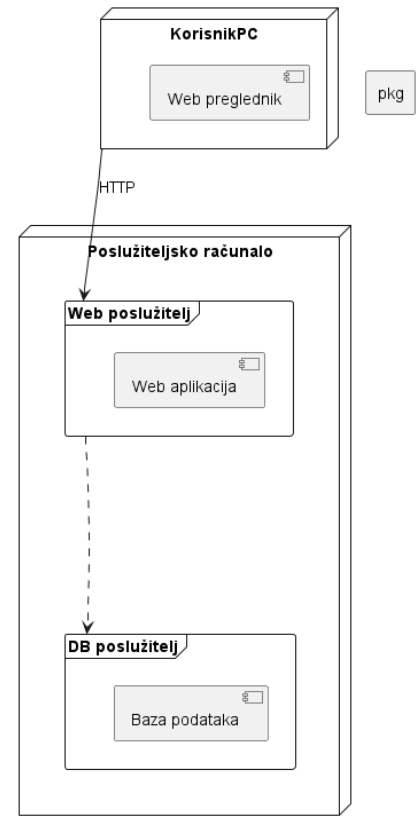
\includegraphics[width=1\linewidth]{dijagrami/dijagramRazmjestanja.png}
	        \centering
	        \caption{Prikaz dijagrama razmještanja}
	        \label{fig:Prikaz dijagrama razmještanja}
        \end{figure}

			\eject 
		
		\section{Upute za puštanje u pogon}

		Za postavljanje aplikacije u produkcijsko okruženje, ključno je implementirati sve komponente na GitHub platformi. Ovaj korak je presudan jer omogućava kreiranje Docker kontejnera, koji su esencijalni za funkcionalnost aplikacije u radnom okruženju. Izvorni kod naše aplikacije dostupan je na https://github.com/KvesaFer/Codeblaze.

		Implementaciju aplikacije izvodimo kroz Render, cloud-based platformu-as-a-service (PaaS). Render nudi potrebnu infrastrukturu za pokretanje aplikacije. Prije početka rada na Render platformi, neophodno je u korijenskom direktoriju izvornog koda kreirati 'render.yaml' datoteku. Ova datoteka služi kao 'Blueprint spec', konfiguracijski set za implementaciju i aktivaciju aplikacije na Render platformi.

		U 'render.yaml' datoteci definiramo tri ključna servisa naše aplikacije: 'server', 'client', i 'db'. Svaki servis, osim PostgreSQL baze, treba sadržavati atribute 'type', 'name', i 'env'. Za PostgreSQL bazu, potrebno je navesti samo 'name', a detalji implementacije su već dostupni kroz predefiniranu uslugu na Render platformi.

		Dodatno, definiramo svojstva za preostale servise - frontend i backend. Atribut 'env' određuje okruženje izvođenja i postavljen je na 'Docker', što omogućava izgradnju aplikacije kroz Docker kontejnere. Svaki definirani servis predstavlja zasebnu 'Docker image' datoteku, koja uključuje kod, alate, biblioteke i ostale postavke potrebne za izgradnju kontejnera.

		Za svaki servis, 'repo' svojstvo postavljamo na putanju GitHub repozitorija s izvornim kodom aplikacije. Također, definiramo 'branch' svojstvo na 'main' granu i 'rootDir' za određivanje korijenskog direktorija repozitorija. 'BuildFilter' svojstvo omogućava definiranje putanje do datoteka čije promjene na 'main' grani iniciraju redeployment servisa.

		Za postavljanje varijabli okruženja, koristimo mogućnost definiranja zavisnosti varijabli jednog servisa o svojstvima već postojećih Render servisa. Varijable okruženja za 'backend' servis povezan s bazom podataka dohvaćamo preko definiranih svojstava Render servisa za PostgreSQL bazu. Ostale varijable, koje su privatne, postavljamo direktno na Render platformu.

		Kreiranje korisničkog računa i prijava na https://dashboard.render.com/ su prvi koraci za korištenje platforme. Nakon toga, odabiremo 'Blueprints' i 'New Blueprint Instance', birajući repozitorij i granu s našim 'render.yaml' datotekom. Render omogućava povezivanje s GitHub računom i odabir repozitorija.

		Nakon spremanja promjena, Render web aplikacija postaje povezana s repozitorijem koji sadrži izvorni kod i 'render.yaml' datoteku. Na osnovu definirane konfiguracije, Render potom pokreće aplikaciju u radno okruženje.

		Konačna verzija aplikacije dostupna je na URL-u koji se generira nakon uspješnog deploya na Render platformi. Važno je napomenuti da, u skladu s uputama za deploy, potrebno je uključiti specifične konfiguracijske korake. To uključuje dodavanje Dockerfile-a, koji se nalazi u 'docker' direktoriju, sa specifičnim verzijama za Maven i Gradle. Također, preporučuje se postavljanje 'server.servlet.context-path' na '/api' u 'application.properties' za backend zahtjeve.

		Za lokalni razvoj, koristeći Liquibase i H2 bazu, preporuča se dodavanje odgovarajućih dependency-a u 'pom.xml' i kreiranje 'application-dev.properties' za lokalni dev profil. Ovo olakšava razvoj i testiranje aplikacije. Važno je paziti na promjene nad bazom, gdje se promjene nad changelogovima ne smiju mijenjati jednom kada su deployani.

		Kreiranje baze podataka na Renderu uključuje postavljanje imena baze te postavljanje opcionalnog korisničkog imena, dok je lozinka automatski generirana. Također, konfiguracija backenda i frontenda na Renderu zahtijeva povezivanje GitHub računa, odabir projekta, postavljanje environment varijabli, i konfiguraciju Dockerfile-a.

		Za deploy frontenda, koraci uključuju dodavanje potrebnih dependency-a u 'package.json', konfiguraciju proxy servera, i postavljanje build i start skripti. Konačno, aplikacija će biti dostupna na URL-u koji se generira nakon deploya na Render platformi.

		Konačna aplikacija dostupna je na poveznici:

		\eject
	\chapter{Zaključak i budući rad}
		
		\textbf{\textit{dio 2. revizije}}\\
		
		 \textit{U ovom poglavlju potrebno je napisati osvrt na vrijeme izrade projektnog zadatka, koji su tehnički izazovi prepoznati, jesu li riješeni ili kako bi mogli biti riješeni, koja su znanja stečena pri izradi projekta, koja bi znanja bila posebno potrebna za brže i kvalitetnije ostvarenje projekta i koje bi bile perspektive za nastavak rada u projektnoj grupi.}
		
		 \textit{Potrebno je točno popisati funkcionalnosti koje nisu implementirane u ostvarenoj aplikaciji.}
		
		\eject 
	\chapter*{Popis literature}
		\addcontentsline{toc}{chapter}{Popis literature}
	 	
 		
		
		\begin{enumerate}
			
			
			\item  Programsko inženjerstvo, FER ZEMRIS, \url{http://www.fer.hr/predmet/proinz}
			
			
		\end{enumerate}
		
		 
	
	
	\begingroup
	\renewcommand*\listfigurename{Indeks slika i dijagrama}
	%\renewcommand*\listtablename{Indeks tablica}
	%\let\clearpage\relax
	\listoffigures
	%\vspace{10mm}
	%\listoftables
	\endgroup
	\addcontentsline{toc}{chapter}{Indeks slika i dijagrama}


	
	\eject 
		
	\chapter*{Dodatak: Prikaz aktivnosti grupe}
		\addcontentsline{toc}{chapter}{Dodatak: Prikaz aktivnosti grupe}
		
		\section*{Dnevnik sastajanja}
		
		\begin{packed_enum}
			\item  sastanak
			
			\item[] \begin{packed_item}
				\item Datum: 20. listopada 2023.
				\item Prisustvovali: M. Kvesić, M. Jakovac, M. Knez, K. Šoštar, K. Đuroković, J. Gunjača, M. Bušić
				\item Teme sastanka:
				\begin{packed_item}
					\item  upoznavanje članova tima
					\item  proučavanje zadatka
					\item  podjela prvih zadataka
					\item  postavljanje GitHuba 
					\item  napravljen početni plan projekta
				\end{packed_item}
			\end{packed_item}
			
			\item  sastanak
			\item[] \begin{packed_item}
				\item Datum: 25. listopada 2023.
				\item Prisustvovali: M. Kvesić, M. Jakovac, M. Knez, K. Šoštar, K. Đuroković, J. Gunjača, M. Bušić
				\item Teme sastanka:
				\begin{packed_item}
					\item  komentiranje obavljenih zadataka
					\item  rasprava o sljedećim koracima
					\item  napravljena skica projekta
					\item  podjela novih zadataka
				\end{packed_item}
			\end{packed_item}
			
			\item  sastanak
			\item[] \begin{packed_item}
				\item Datum: 04. studenoga 2023.
				\item Prisustvovali: M. Kvesić, M. Jakovac, M. Knez, K. Šoštar, K. Đuroković, J. Gunjača, M. Bušić
				\item Teme sastanka:
				\begin{packed_item}
					\item  komentiranje obavljenih zadataka
					\item  detaljna analiza i popravak postojećih obrazaca uporabe
					\item  analiza baze podataka
					\item  podjela novih zadataka
				\end{packed_item}
			\end{packed_item}
			
			\item  sastanak
			\item[] \begin{packed_item}
				\item Datum: 11. studenoga 2023.
				\item Prisustvovali: M. Kvesić, M. Jakovac, M. Knez, K. Šoštar, K. Đuroković, J. Gunjača, M. Bušić
				\item Teme sastanka:
				\begin{packed_item}
					\item  komentiranje obavljenih zadataka
					\item  dogovoren plan za prvu reviziju
					\item  rasprava o nedoumicama oko aplikacije
					\item  dogovoren popravak dokumentacije
					\item  testiranje napravljene aplikacije
					\item  podjela novih zadataka
				\end{packed_item}
			\end{packed_item}
			
			\item  sastanak
			\item[] \begin{packed_item}
				\item Datum: 17. studenoga 2023.
				\item Prisustvovali: M. Kvesić, M. Jakovac, M. Knez, K. Šoštar, K. Đuroković, J. Gunjača, M. Bušić
				\item Teme sastanka:
				\begin{packed_item}
					\item  provjera dokumentacije za prvu predaju
				\end{packed_item}
			\end{packed_item}
			
			\item  sastanak
			\item[] \begin{packed_item}
				\item Datum: 1. prosinca 2023.
				\item Prisustvovali: M. Kvesić, M. Jakovac, M. Knez, K. Šoštar, K. Đuroković, J. Gunjača, M. Bušić
				\item Teme sastanka:
				\begin{packed_item}
					\item  razrada plana za daljnji razvoj aplikacije
					\item  podjela u podtimove
					\item  podjela zadataka
				\end{packed_item}
			\end{packed_item}
			
			\item  sastanak
			\item[] \begin{packed_item}
				\item Datum: 15. prosinca 2023.
				\item Prisustvovali: M. Kvesić, M. Jakovac, M. Knez, K. Šoštar, K. Đuroković, J. Gunjača, M. Bušić
				\item Teme sastanka:
				\begin{packed_item}
					\item  diskutiranje nedoumica
					\item  testiranje postojećih funkcionalnosti
				\end{packed_item}
			\end{packed_item}
			
			\item  sastanak
			\item[] \begin{packed_item}
				\item Datum: 22. prosinca 2023.
				\item Prisustvovali: M. Kvesić, M. Jakovac, M. Knez, K. Šoštar, K. Đuroković, J. Gunjača, M. Bušić
				\item Teme sastanka:
				\begin{packed_item}
					\item  podjela preostalih zadataka
				\end{packed_item}
			\end{packed_item}
			
			\item  sastanak
			\item[] \begin{packed_item}
				\item Datum: 12. siječnja 2024.
				\item Prisustvovali: M. Kvesić, M. Jakovac, M. Knez, K. Šoštar, K. Đuroković, J. Gunjača, M. Bušić
				\item Teme sastanka:
				\begin{packed_item}
					\item  pregled svega napravljenog
					\item  dogovor oko izrade preostalog dijela dokumentacije
				\end{packed_item}
			\end{packed_item}
			\item  sastanak
			\item[] \begin{packed_item}
				\item Datum: 15. studenoga 2024.
				\item Prisustvovali: M. Kvesić, M. Jakovac, M. Knez, K. Šoštar, K. Đuroković, J. Gunjača, M. Bušić
				\item Teme sastanka:
				\begin{packed_item}
					\item  završetak implementacije
				\end{packed_item}
			\end{packed_item}
			
			 
			
			%
			
		\end{packed_enum}
		
		\eject
		\section*{Tablica aktivnosti}
		

			\begin{longtblr}[
					label=none,
				]{
					vlines,hlines,
					width = \textwidth,
					colspec={X[7, l]X[1, c]X[1, c]X[1, c]X[1, c]X[1, c]X[1, c]X[1, c]}, 
					vline{1} = {1}{text=\clap{}},
					hline{1} = {1}{text=\clap{}},
					rowhead = 1,
				} 
			
				\SetCell[c=1]{c}{} & \SetCell[c=1]{c}{\rotatebox{90}{\textbf{Marin Kvesić }}} & \SetCell[c=1]{c}{\rotatebox{90}{\textbf{Matija Jakovac }}} &	\SetCell[c=1]{c}{\rotatebox{90}{\textbf{Mirna Knez }}} & \SetCell[c=1]{c}{\rotatebox{90}{\textbf{Jerko Gunjača }}} &	\SetCell[c=1]{c}{\rotatebox{90}{\textbf{Karla Šoštar }}} & \SetCell[c=1]{c}{\rotatebox{90}{\textbf{Katarina Đuroković }}} &	\SetCell[c=1]{c}{\rotatebox{90}{\textbf{Matea Bušić }}} \\  
				Upravljanje projektom 		&24 &21 &12 &14 &11 &11 &15 \\
				Opis projektnog zadatka 	&0  &0  &0  &0  &0  &0  &13 \\ 
				
				Funkcionalni zahtjevi       &0  &0  &0  &0  &6  &6  &5 \\ 
				Opis pojedinih obrazaca 	&0 &0  &0  &0  &9  &15  &7  \\
				Dijagram obrazaca 			&0  &0  &0  &0  &7  &8  &0  \\ 
				Sekvencijski dijagrami 		&0  &0  &0  &0  &5  &7  &0  \\
				Opis ostalih zahtjeva 		&0  &0  &0  &0  &0  &0  &1  \\ 

				Arhitektura i dizajn sustava  &0  &0  &13 &0  &0  &0  &2   \\ 
				Baza podataka				&0  &0  &9  &0  &0  &0  &0   \\ 
				Dijagram razreda 			&0  &0  &6  &0  &0  &2 &0   \\
				Dijagram stanja				&0  &0  &0  &0  &0  &2  &0  \\
				Dijagram aktivnosti 		&0  &0  &0  &0  &0  &1  &0  \\
				Dijagram komponenti			&0  &0  &0  &0  &0  &0  &5  \\ 
				Korištene tehnologije i alati 		&0  &0  &0  &0  &0  &0  &0  \\ 
				Ispitivanje programskog rješenja 	&0  &0  &0  &0  &18  &0  &0  \\
				Dijagram razmještaja			&0  &0  &3  &0  &0  &0  &0  \\
				Upute za puštanje u pogon 		&0  &0  &5  &0  &0  &0  &0  \\
				Dnevnik sastajanja 			&0  &0  &0  &0  &0  &0  &2  \\ 
				Zaključak i budući rad 		&0  &0  &0  &0  &0  &0  &2  \\  
				Popis literature 			&0  &0  &0  &0  &0  &0  &1  \\  
			
			
				Izrada početne stranice 				&5  &3  &8  &14  &0  &0  &5  \\
				Izrada baze podataka 		 			&6  &14  &3  &0  &0  &0  &0 \\
				Spajanje s bazom podataka 							&6  &5  &0  &0  &0  &0  &0  \\
				Back end 							&63  &65  &2  &0  &40  &15  &35  \\
				Front end							&50  &45  &70  &60  &20  &45  &25  \\
				Postavljanje web aplikacije na poslužitelj							&5  &5  &0  &0  &0  &0  &0  \\
				 						
			\end{longtblr}
					
					
		\eject
		\section*{Dijagrami pregleda promjena}
		
		\textbf{\textit{dio 2. revizije}}\\
		
		\textit{Prenijeti dijagram pregleda promjena nad datotekama projekta. Potrebno je na kraju projekta generirane grafove s gitlaba prenijeti u ovo poglavlje dokumentacije. Dijagrami za vlastiti projekt se mogu preuzeti s gitlab.com stranice, u izborniku Repository, pritiskom na stavku Contributors.}
		
	



\end{document} %naredbe i tekst nakon ove naredbe ne ulaze u izgrađen dokument 


